\chapter{Coronal Dimming Case Studies}
\label{chaptercasestudy}

% Mini-abstract
This chapter focuses on the detailed analysis of two coronal dimming events. One was selected for its relative simplicity, involving only mass-loss dimming and some thermal effects, while the other was selected for its complexity, involving nearly all of the types of dimming as described in Chapter \ref{chaptermechanisms}. Observations and analysis of the EUV irradiance and images of these events as well as the related coronagraphs are first described in Section \ref{sec:observations}. A new method for deconvolving flare emission from dimming irradiance measurements is developed in Section \ref{sec:deconvolve} while Section \ref{sec:deconvolveerrors} contains the associated error propagation. Finally, Section \ref{sec:casestudyresults} provides analyses spanning the observations of these two coronal dimming events and parameterizes dimming into depth and slope. We find that the new deconvolution method for irradiance successfully matches the dimming profile extracted from the spatially-isolated dimming as obtained from EUV image time series for the simpler dimming case. Thus, we show that it is possible to accurately characterize dimming in a localized area even with no spatial resolution. Further analysis of the complex dimming will be required to isolate mass-loss from the full-range of cotemporal dimming processes, which will be a topic of postdoctoral research. The preliminary analyses of this more complex dimming are provided here. 

\section{Observations and Analysis}
\label{sec:observations}

\subsection{Simple Dimming Case}
\label{sec:observationssimple}
This event occurred on 2010 August 7 at approximately 18:24 UT. The eruptive event consisted of an M1.0 flare, dimming in the region around the flare, and a coronal mass ejection (CME). Other, relatively distant, active regions were also on disk but did not have any significant sympathetic responses. Mass-loss dimming and flare-related thermal effects were found to be important, while the other type of dimming (see Chapter \ref{chaptermechanisms}) were negligible. 

\paragraph{Coronagraph Observations}

\begin{figure}[!h]
    \begin{center}
	    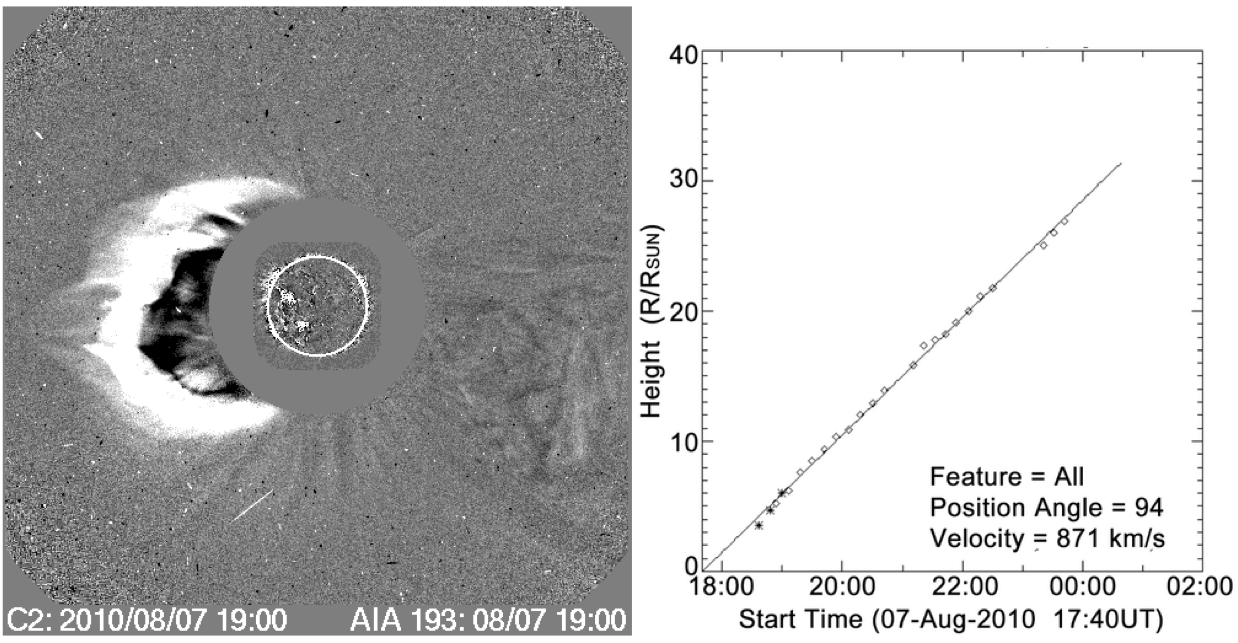
\includegraphics[width=150mm]{Images/Lasco2010Aug7Cme.png}
    \end{center}
    \caption[LASCO coronagraph data for 2010 August 7 event]{
        CME event at 19:00 on 2010 August 7. Left: difference image from LASCO C2 and AIA 193 \AA\ channel. 
        Right: CME height versus time shows nearly linear velocity of 871 $km\ s^{-1}$. 
        Figure adapted from CDAW CME Catalog, courtesy of S. Yashiro and N. Gopalswamy.
	}
    \label{lasco2010aug7}
\end{figure}

The Coordinated Data Analysis Workshops (CDAW) LASCO CME catalog (herein referred to simply as the CDAW catalog) is an extensive database of all CMEs observed by the SOHO/LASCO coronagraphs with related quantities such as date, time, computed velocity, and sometimes mass \citep{Gopalswamy2009}. The CDAW catalog has seven CME events listed for 2010 August 7. All but two of them occur prior to the M1.0 flare at 18:24 UT that is of primary interest for the present study. This rules out all but those two to be CMEs associated with the M1.0 flare. The CME shown in Figure \ref{lasco2010aug7} is flagged as a halo event with a time of 18:36 UT in CDAW, while the next event occurred with a central position angle of 116\degree\ at 22:24 UT. The timing and location of the flare and associated dimming region suggest that the halo CME is the one associated with the dimming. The plane-of-sky velocity estimate for this CME is 871 $km\ s^{-1}$ as indicated in Figure \ref{lasco2010aug7}. No mass is listed for this CME in CDAW, but using LASCO and STEREO data and the techniques outlined in \citet{Colaninno2009}, a mass of $6.4 \times 10^{15}$ g was computed for this CME event (A. Vourlidas 2014, private communication). A true space velocity was also computed as 850 $km\ s^{-1}$ at 9 R\astrosun\ with a deceleration of 6.84 $m\ s^{-2}$ (Figure \ref{stereo2010aug7}). Based on these estimates for mass and velocity, this CME is
considered be of modest size.

\begin{figure}[!h]
    \begin{center}
	    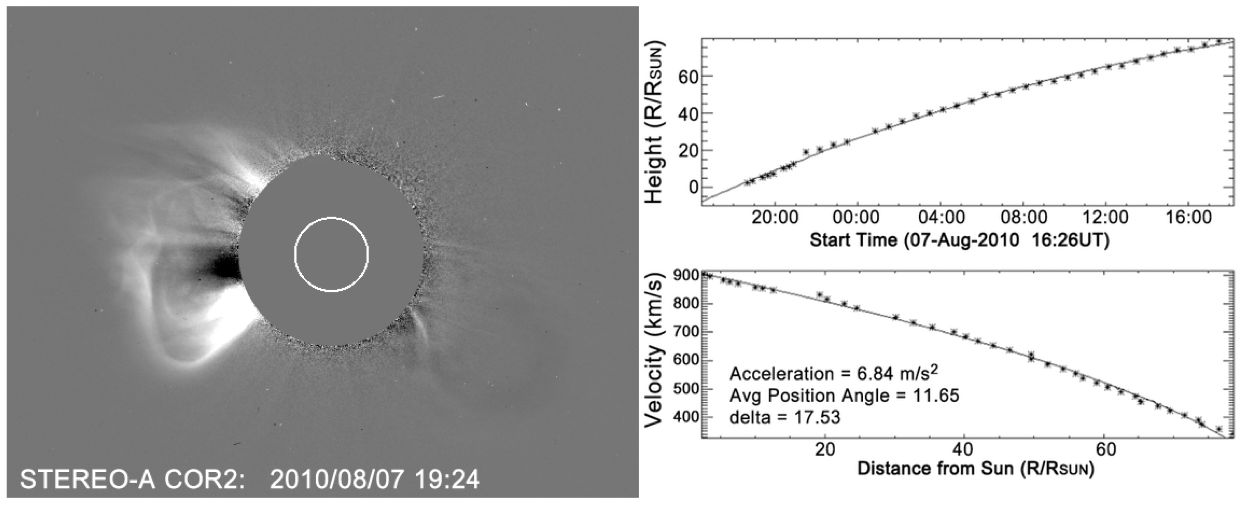
\includegraphics[width=150mm]{Images/Stereo2010Aug7Cme.png}
    \end{center}
    \caption[LASCO coronagraph data for 2010 August 7 event]{
        Left: STEREO-A COR2 difference image at 19:24 UT. Right: CME height vs. time calculated from STEREO and shows a 
        deceleration of 6.84 $m\ s^{-2}$. Figure courtesy of Barbara Thompson. 
	}
    \label{stereo2010aug7}
\end{figure}

\paragraph{SDO/AIA EUV Image Observations}
The relative simplicity of this event is why it was chosen for a case study. The observations in AIA do not suggest that obscuration, waves, or Doppler shift contributed to the observed dimming. The area in the red contour of Figure \ref{aia2010aug7} was selected manually (by eye) to represent the region of mass loss. Pixel values inside each contour were summed and a time series of these sums created with successive images in multiple AIA wavelength bands. These light curves are shown on the right of Figure \ref{aia2010aug7}. The light curve for the red contour shows clear dimming in 193 \AA\ and 171 \AA. In fact, the dimming from this region accounts for nearly all of the observed dimming throughout the entire event. This contour was selected after several iterations that indicated slight deviations in the contour had minimal impact on the light curve, as long as the dark region was fully encompassed. In other words, the result is fairly insensitive to the precise contour selection. The other contours were also selected manually to isolate regions of potential dimming e.g., as a sympathetic response from the solar eruptive event of interest. The exception is the magenta contour surrounding the flare loops that brightens dramatically but does not ever dim. 

\begin{figure}[!h]
    \begin{center}
	    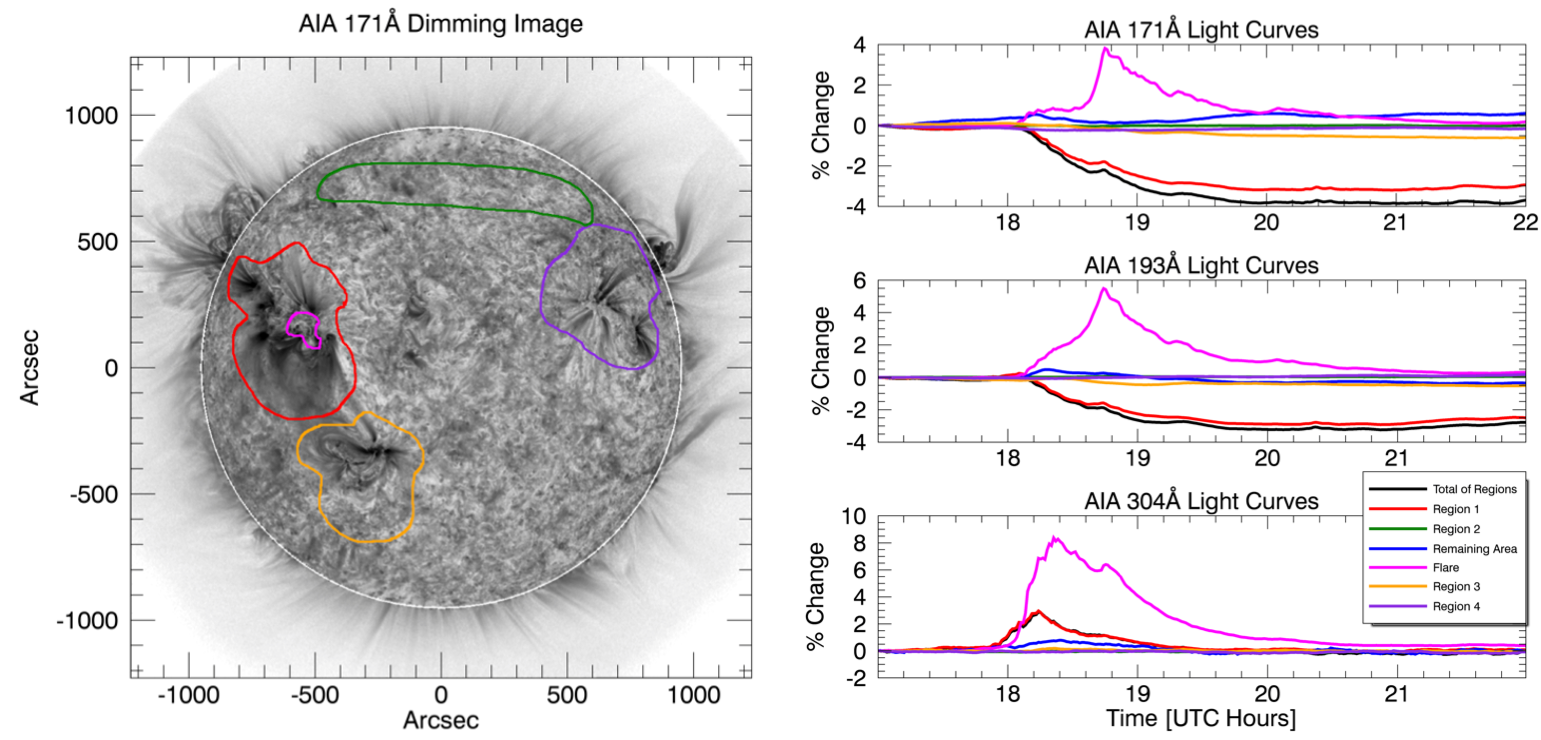
\includegraphics[width=166mm]{Images/Aia2010Aug7.png}
    \end{center}
    \caption[AIA contour analysis for 2010 August 7 event]{
        AIA results for the M1.0 Flare on 2010 August 7. Images improved by using point spread function to compensate for 
        instrument ``blurring" of light. Left: AIA 171 \AA\ channel difference image with subjectively 
        selected region contours overlaid. The red contour outlines what is thought to be the region of mass loss. The 
        orange and purple contours outline other active regions on the disk, which have the potential to have sympathetic 
        dimming. The green contour outlines a filament, which also has the potential to sympathetically dim based on its 
        behavior during the M flare on 2010 August 5. The magenta contour isolates the flaring coronal loops. The white line 
        around the solar limb is an artifact of the solarsoft derotation method. Right three plots: light curves of AIA 171 
        \AA, 193 \AA, and 304 \AA\ channels for the color-corresponding contours on the AIA image. The blue line is the 
        light curve for all on-disk area not enclosed by a contour. The black line is the sum of all contoured regions and 
        acts as a proxy for total dimming. All percent changes are calculated from the band's value at 17:00 UT, prior to 
        the flare. The transition region He 304 \AA\ emission does not show dimming; both corona Fe emissions (171 \AA\ and 
        193 \AA) show dimming.
	}
    \label{aia2010aug7}
\end{figure}

The He II 304 \AA\ light curves are included to provide a contrast to the dimming effects seen in the coronal Fe lines. This He II wavelength is generated primarily in the chromosphere and transition region, as opposed to the coronal source of the other wavelengths. Mass loss occurs primarily in the corona, as the term coronal mass ejection suggests. This is reflected in the lack of dimming observed in the non-coronal He II 304 \AA\ emission line.

\begin{figure}[!h]
    \begin{center}
	    \includegraphics[width=166mm]{Images/AiaComposite2010Aug7.png}
    \end{center}
    \caption[AIA before/after images of 2010 August 7 event]{
	    AIA composite images (a) prior to solar eruptive event and (b) during deep dimming. In these images, purple is 
	    211 \AA, brownish-gold is 193 \AA, and yellow is 171 \AA. These static images show dimming in the region as outlined 
	    in Figure \ref{aia2010aug7}, though the change is much more dramatic and obvious when viewed as a movie. 
	}
    \label{aiacomposite2010aug7}
\end{figure}

Thermal effects may play a role in this event but may be difficult to quantify using only AIA because the relatively wide spectral bands of AIA channels mean many emission lines and continuum are blended together (see Figure \ref{aiabandpasses} and Table \ref{tab:emissionlines}), which makes specifying a well-defined temperature difficult. Nevertheless, some indication of temperature is given by AIA and multi-wavelength composites can aid in this analysis. Figure \ref{aiacomposite2010aug7} shows AIA composite images (211 \& 193 \& 171 \AA) before the solar eruptive event and during the dimming. All of these bands correspond primarily to the corona and transition region. If an area is dark, that means that there is little emission in all three of these wavelengths. Since these three bands span temperatures across at least 0.6-1.86 MK, that is indicative of mass loss. In areas where temperature effects are very strong, e.g., heating in the confined flare loops, it can be seen that emission is strong in all three of these bands resulting in the composite being white. Even though the flare loop region is also where the highest ionization states and their emission can be found, there is still ample emission in these relatively low ionization states of Fe. Thus, it's unlikely that a region in these composites would become dark purely from a temperature change. EVE is less sensitive than AIA to blending in temperature space due to its higher spectral resolution and plethora of emission lines from Fe at different ionization states. A future study using the differential emission measure techniques of \citet{Caspi2014} to study the temperature evolution could help to quantify this effect.

\paragraph{SDO/EVE EUV Irradiance Observations}
Figure \ref{eve2010aug7} shows a trend that is consistent with the findings from Figure \ref{detectedDimmingVsIonization} --that an ion's peak formation temperature\footnote{Recall that greater ionization requires greater energy and that temperature is one measure of energy content for a Maxwellian plasma}is inversely proportional to magnitude of dimming. The transition from an ionization state that shows dimming to ones that only show brightening occurs at Fe XIV 211 \AA, which itself shows dimming in some events but not others. The transition for where the Fe emission shows dimming varies by solar eruptive event. For example, the Fe XVI 335 \AA\ emission has shown dimming for larger CME events \citep{Woods2011}. Herein, we will refer to Fe IX 171 \AA\ through Fe XIV 211 \AA\ as ``dimming lines" and Fe XIV 211 \AA\ through Fe XXIV 192 \AA\ as ``nondimming lines" (note that 211 \AA\ is included in both descriptions to reflect its ambiguity).

It is also important to note in Figure \ref{eve2010aug7} that the onset of dimming in the dimming lines is nearly simultaneous. Meanwhile, the gradual-phase flare peak is delayed in lower ionizations of Fe, which is due to a cooling effect. The primary source of energy release in a flare is near the point of magnetic reconnection, typically far above the footpoints of the magnetic loops involved, in the corona. Some of the energy goes into the acceleration of particles downward. When these particles impact the denser chromosphere, they cause the heating and chromospheric evaporation. As that thermal plasma enters the corona it cools \citep{Fletcher2011}, and highly ionized Fe gains electrons. Thus, the peak is later for lower ionization states in this case as seen in Figure \ref{eve2010aug7}. The Fe IX 171 \AA\ irradiance, in particular, shows the competing effects of this gradual phase flare peak and coronal dimming: it's irradiance begins to drop at the same onset as the other emission lines, then has a positive peak of about +2\%, and drops to a dimmed condition again. Images with spatial resolution can isolate the flaring region responsible for this peak, as is shown with the magenta contour in Figure \ref{aia2010aug7}. Alternatively, we have developed a method for isolating and removing this peak in dimming lines with the spatially-integrated irradiance from EVE, which will be detailed in Section \ref{sec:deconvolve}. 

\newpage
\begin{singlespace}
\begin{figure}[H]
    \begin{center}
	    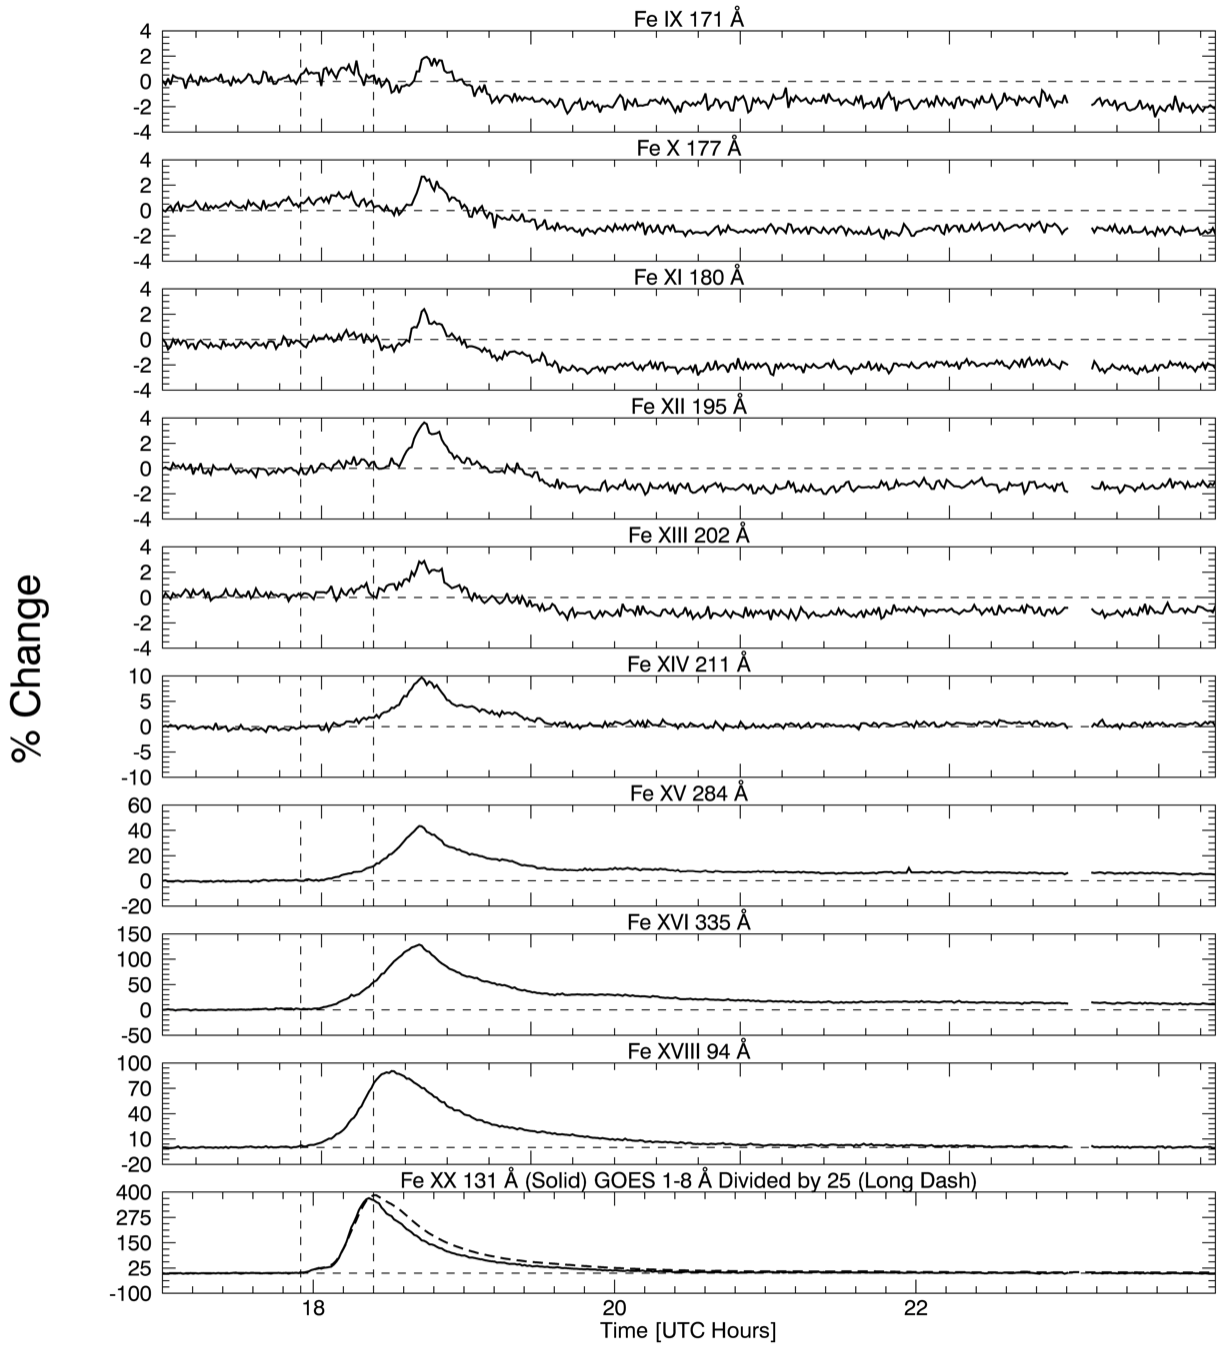
\includegraphics[width=166mm]{Images/Eve2010Aug7.png}
    \end{center}
    \caption[EVE selected extracted emission lines for 2010 August 7 event]{ 
        One minute average EVE light curves of the 2010 August 7 coronal dimming event for most of the spectral lines listed 
        in Table \ref{tab:emissionlines}, as well as the GOES 1-8 \AA\ channel light curve. The leftmost vertical dashed 
        line indicates
        the GOES event start time, while the other vertical dashed line indicates the GOES event peak time. Peak formation 
        temperature of the EVE spectral lines increases from top to bottom plot. Fe IX to Fe XIII show clear dimming, Fe XIV
        is borderline, and Fe XV to Fe XX show smooth brightening with no dimming. The Fe XX 131 \AA\ profile is very 
        similar to GOES 1-8 \AA, indicating that this line in EVE is a good proxy for gradual phase timing. Also note the 
        vertical axes: dimming is on the order of a few percent for the cooler Fe emissions while the hotter Fe emissions 
        have bright peaks in the hundreds of percent. All percent changes are calculated from the spectral irradiance at 
        17:00 UT.
    }
    \label{eve2010aug7}
\end{figure}
\end{singlespace}

\subsection{Complex Dimming Case}
This event occurred on 2011 August 4 at approximately 3:47 UT. It spawned from NOAA active region 11261 at location N19W36. The eruptive event consisted of an M9.3 flare, a large and fast CME, and nearly all of the types of dimming discussed in Chapter \ref{chaptermechanisms}: mass-loss and thermal dimming, a global wave that then triggered a sympathetic filament eruption, and an obscuration dimming from the filament. No bandpass or Doppler dimming were identified even in this relatively energetic event. This event was chosen specifically for presenting so many types of dimming and related physical processes in a single case. 

\paragraph{Coronagraph Observations}

\begin{figure}[!h]
    \begin{center}
	    \includegraphics[width=140mm]{Images/Coronagraphs2011Aug4.png}
    \end{center}
    \caption[LASCO and STEREO coronagraph data for 2011 August 4 event]{ 
        Coronagraph images of CME associated with 2011 August 4 dimming event. 
        From left to right the coronagraphs are STEREO Behind C2, LASCO C3, and STEREO Ahead C2. Top: Images prior to CME. 
        Bottom: Images during CME. 
    }
    \label{coronagraphs2011aug4}
\end{figure}

Images from the three coronagraphs are shown in Figure \ref{coronagraphs2011aug4}. The CME in Figure \ref{coronagraphs2011aug4} (b) can be seen in STEREO-B (behind) on the right of the solar disk, in LASCO as the start of a halo CME offset to the upper-right of the disk, and in STEREO-A (ahead) on the left of the disk. Additionally, bright streamers can be seen inside the CME and on the opposite side of the Sun, signifying that the outer corona of the Sun was also in a more complex configuration than the 2010 August 7 case. 

The CDAW catalog for this event lists it as a halo CME with a velocity of 1315 $km\ s^{-1}$, relatively fast for a CME (faster than 99.03\% of other CMEs, see Figure \ref{fig:cmespeeds1315}), and a mass of $1.16 \times 10^{16}\ g$. However, halo CMEs present a strong challenge for obtaining accurate mass, and the catalog flags it as a poor mass estimate. Mass estimates based on the three coronagraphs are $8.6 \times 10^{15}\ g$ for LASCO C3 (35\% lower than the CDAW value), $7-8 \times 10^{15}\ g$ for STEREO-A COR2, and $4.3 \times 10^{15}\ g$ for STEREO-B COR2 (A. Vourlidas 2013, private communication). A deprojected, 3-D analysis has not been performed for this CME. 

\begin{figure}[!h]
    \begin{center}
	    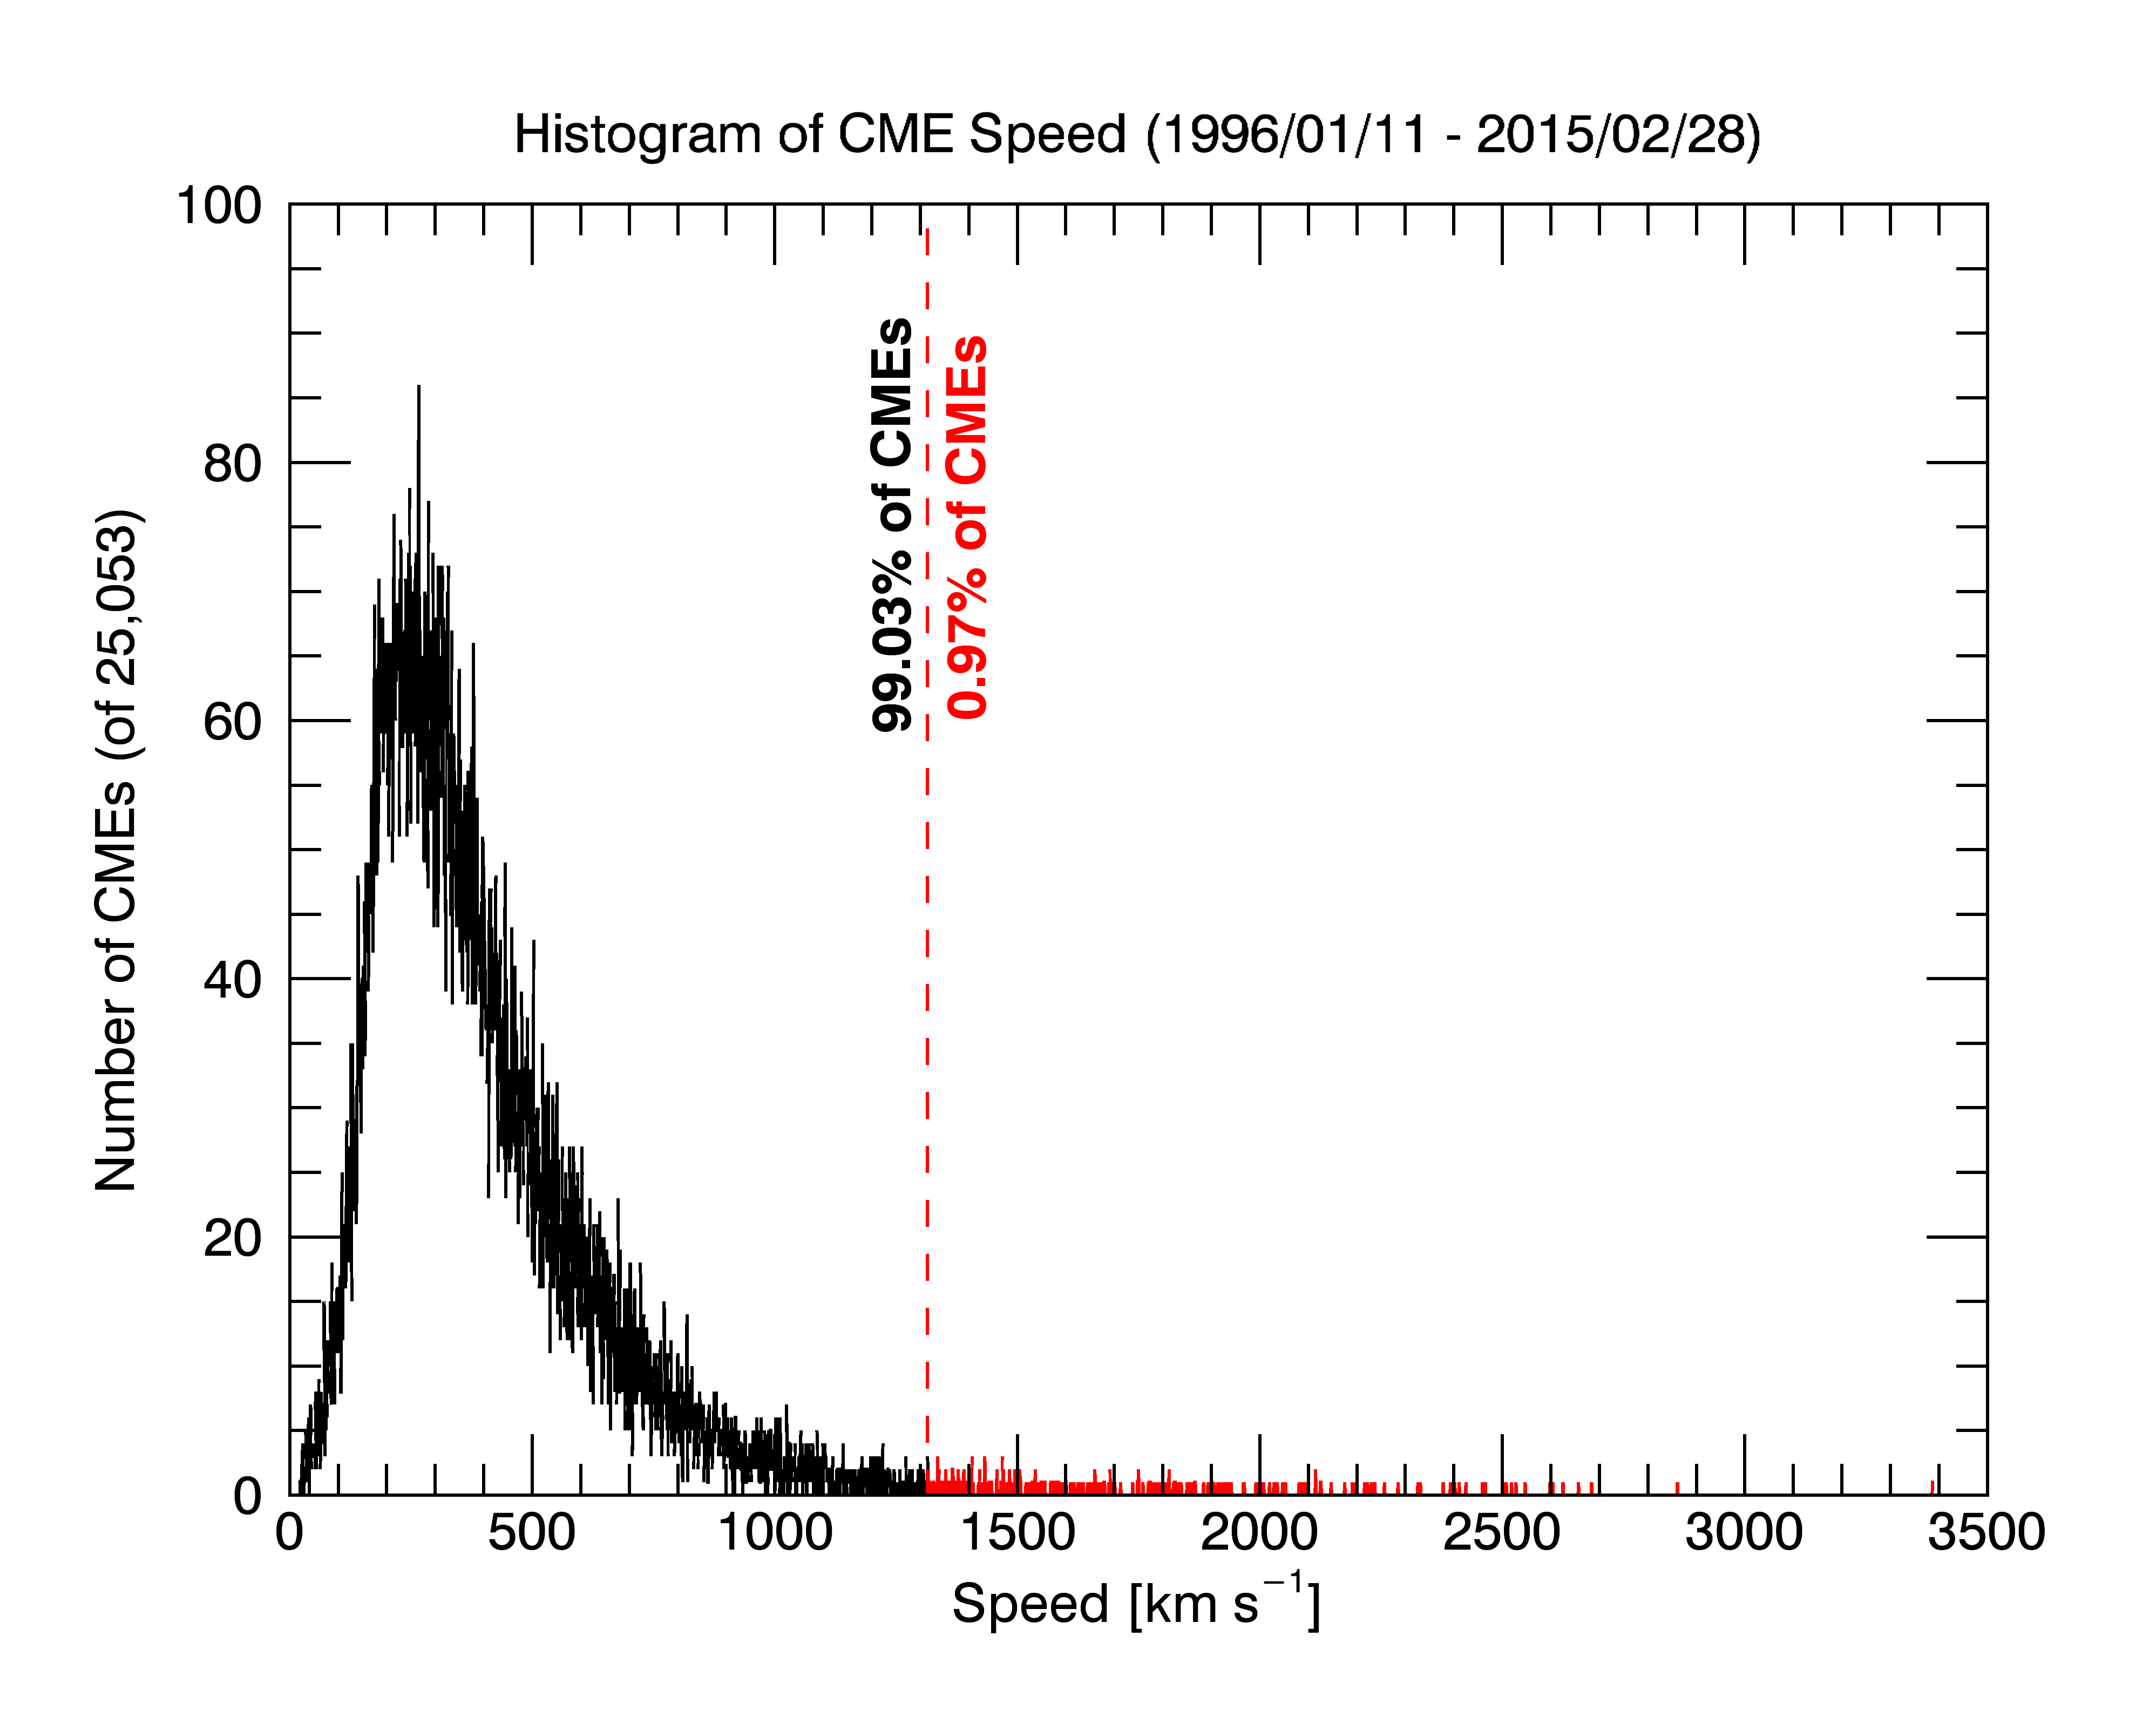
\includegraphics[width=100mm]{Images/HistoricalCmeVelocity.png}
    \end{center}
    \caption[Historical CME speed histogram]{
        Histogram of CME speed from 1995 to 2015 based on the CDAW LASCO CME catalog's 25,053 CMEs with listed speeds. 
        The red vertical line is at 1315 $km\ s^{-1}$, the listed speed of the 2011 August 4 event. 
	}
    \label{fig:cmespeeds1315}
\end{figure}


\paragraph{SDO/AIA EUV Image Observations}

\begin{figure}[!h]
    \begin{center}
	    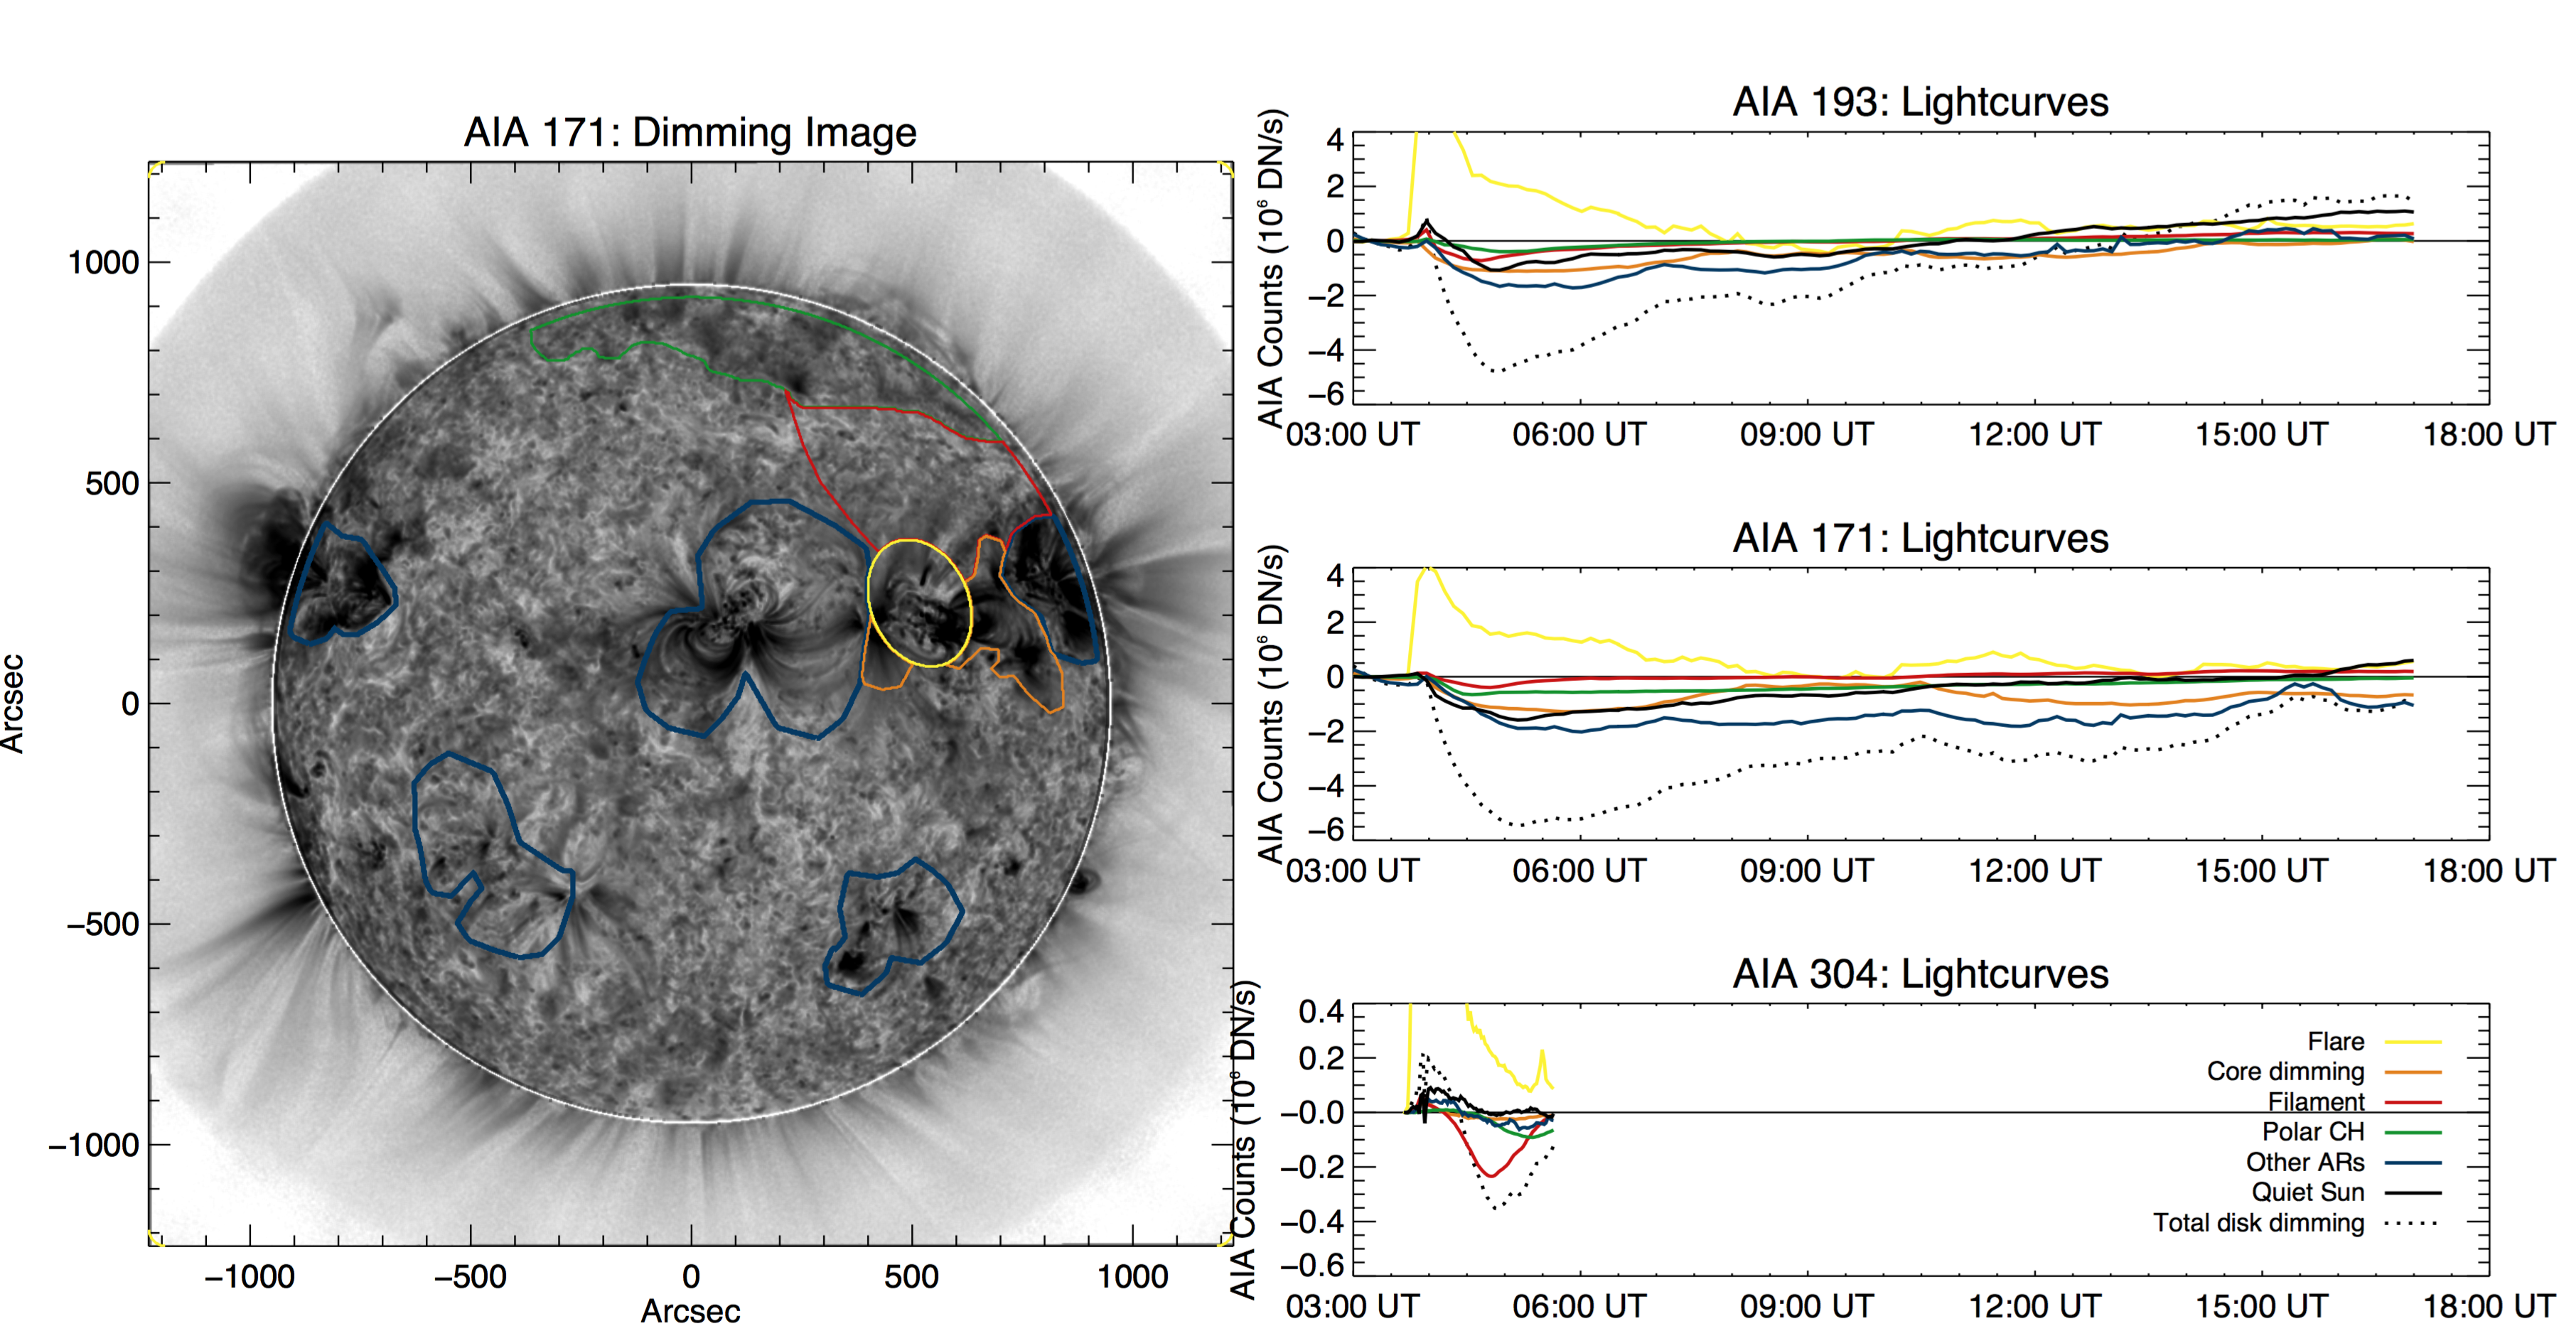
\includegraphics[width=166mm]{Images/Aia2011Aug4.png}
    \end{center}
    \caption[AIA contour analysis for 2011 August 4 event]{
        Same as Figure \ref{aia2010aug7} but for 2010 August 7 event. Colored contours and lines in plots correspond 
        according to legend, but are different from Figure \ref{aia2010aug7}. An additional difference is that the He II
        304 \AA\ line now shows dimming. Not all 304 \AA\ data were available at the time of processing, which is why the 
        time series ends at 6:00 UT. Figure courtesy of Rachel Hock. 
	}
    \label{aia2011aug4}
\end{figure}

The complexities of this eruptive event are quite apparent in AIA observations. Figure \ref{aia2011aug4} is in the same format as Figure \ref{aia2010aug7} but is for the 2011 August 4 event. Dimming is seen in numerous locations for this event, indicating the far-reaching influence of this eruption. In particular, even though 304 \AA\ data were not processed to the end of the dimming window\footnote{Figure \ref{aia2011aug4newregions} shows these data in full, though for differently selected contours}, the main phase of obscuration dimming is clearly visible. Additionally, 193 \AA\ and 171 \AA\ show dimming in every region outside of the flare-isolating contour (yellow). The primary region thought to be associated with mass-loss dimming is labeled ``core dimming" (orange) here. It corresponds to an area immediately surrounding the active region where the flare took place and is bounded by quiet-Sun on top and bottom and other active region loops to the left and right. All other active regions visible on disk are contained in blue contours and eventually show even greater dimming than the core region (orange). Note that for the first several minutes, the core dimming dominates the other active regions. Also, the dotted black dash line is the disk signal excluding the flare region (yellow), effectively the sum of all plotted lines except yellow. It can be seen that the relative contribution of each region to the total dimming is nonzero. Table \ref{tab:aia2011aug4} details these contributions. 

\begin{table}
\small
\caption[2011 August 4 event statistics]{
    Statistics for dimming features in Figure \ref{aia2011aug4} for 2011 August 4 event. Table courtesy of Rachel Hock. 
}
\begin{center}
\rotatebox{90}{
\begin{tabular}{r|rrr|rrr|r@{-}r}
\multicolumn{1}{c|}{\multirow{3}{*}{Dimming Feature}}& \multicolumn{3}{c|}{Count Minimum} & \multicolumn{3}{c|}{Contribution Maximum} & \multicolumn{2}{c}{Range of} \\
& \multicolumn{1}{c|}{Time} & \multicolumn{1}{c|}{Counts} & \multicolumn{1}{c|}{Contribution} & \multicolumn{1}{c|}{Time} & \multicolumn{1}{c|}{Counts} & \multicolumn{1}{c|}{Contribution} & \multicolumn{2}{c}{Contribution}\\
& \multicolumn{1}{c|}{(UT)} & \multicolumn{1}{c|}{($10^6\ DN\ s^{-1}$)} & \multicolumn{1}{c|}{(\%)} & \multicolumn{1}{c|}{(UT)} & \multicolumn{1}{c|}{($10^6\ DN\ s^{-1}$)} & \multicolumn{1}{c|}{(\%)} & \multicolumn{2}{c}{(\%)} \\
\hline \hline
\multicolumn{1}{l}{AIA 193:} \\
\hline
Total disk dimming & 4:55 & -4.81 & & & & & \\
Core dimming & 5:17 & -1.11 & 25.3 & 04:05 & -0.63 & 73.1 & 18.9 & 73.1 \\
Filament eruption & 4:41 & -0.72 & 16.2 & 04:05 & -0.23 & 27.2 &  1.0 & 27.2 \\
Polar coronal hole & 5:03 & -0.39 & 8.5 & 05:17 & -0.38 & 8.7 &  0.6 & 8.7 \\
Non-flaring active regions & 5:53 & -1.72 & 43.1 & 08:04 & -1.05 & 54.6 & 29.6 & 54.6 \\
Quiet Sun & 4:55 & -1.07 & 22.3 & 08:40 & -0.57 & 26.0 &  8.0 & 26.0 \\
\multicolumn{1}{l}{AIA 171:} \\
\hline
Total disk dimming & 5:10 & -5.46 & & & & & \\
Core dimming & 5:53 & -1.28 & 24.5 & 04:05 & -0.40 & 27.3 &  9.4 & 27.3 \\
Filament eruption & 4:48 & -0.40 & 8.0 & 04:41 & -0.38 & 8.1 &  0.0 & 8.1 \\
Polar coronal hole & 4:34 & -0.66 & 15.7 & 04:26 & -0.63 & 16.6 &  7.5 & 16.6 \\
Non-flaring active regions & 6:00 & -2.02 & 38.9 & 08:54 & -1.72 & 53.9 & 16.6 & 53.9 \\
Quiet Sun & 5:10 & -1.59 & 29.0 & 04:05 & -0.68 & 46.7 & 20.8 & 46.7 \\
\multicolumn{1}{l}{AIA 304:} \\
\hline
Total disk dimming & 4:53 & -0.36 & & & & & \\
Core dimming & 5:08 & -0.03 & 9.5 & 04:23 & -0.02 & 62.2 &  7.4 & 62.2 \\
Filament eruption & 4:49 & -0.24 & 69.4 & 04:25 & -0.08 & 304.3 &  9.4 & 304.3 \\
Polar coronal hole & 5:22 & -0.09 & 40.0 & 05:38 & -0.06 & 49.3 &  1.1 & 49.3 \\
Non-flaring active regions & 5:11 & -0.06 & 20.6 & 05:31 & -0.05 & 25.1 &  2.4 & 25.1 \\
Quiet Sun & 5:34 & -0.02 & 14.0 & 05:37 & -0.02 & 14.4 &  0.1 & 14.4 \\
\hline
\end{tabular}
}
\end{center}
\label{tab:aia2011aug4}
\end{table}

The overall structure of Table \ref{tab:aia2011aug4} is wavelength and feature (vertical) and contribution at maximum dimming (i.e. minimum count), maximum dimming contribution, and the range of contributions. It can be seen that in 193 \AA\ and 171 \AA, peak dimming is dominated by the non-flaring active regions. As will be shown later, this is mainly a reflection of the most nearby active region's dimming. It is also worth noting that core dimming reaches its maximum dimming 36 minutes earlier than non-flaring active regions. This suggests that the latter is either a sympathetic response to the primary dimming catalyzed by the global wave or additional mass being ejected that becomes the tail side of the CME. As expected, in 304 \AA, the minimum count is dominated by the filament (red). This is consistent with the physical theory for obscuration dimming detailed in Section \ref{obscurationDimming}. The dominant region changes when looking at the maximum contribution. Here, core dimming dominates for 193 \AA\ but the non-flaring active regions still dominate in 171 \AA. Again, we will soon show that the most nearby active region contributes greatly to the dimming and may have contributed to the outgoing mass of the CME. 304 \AA\ remains consistent for contribution maximum, with its greatest value coming from the filament eruption. Finally, the range of contributions shows that in 193 \AA, core dimming and non-flaring active regions are comparable in their dominance; 171 \AA has greater contribution from non-flaring active regions and the quiet-Sun; and 304 \AA\ is very clearly dominated by the filament. 

\begin{figure}[!h]
    \begin{center}
	    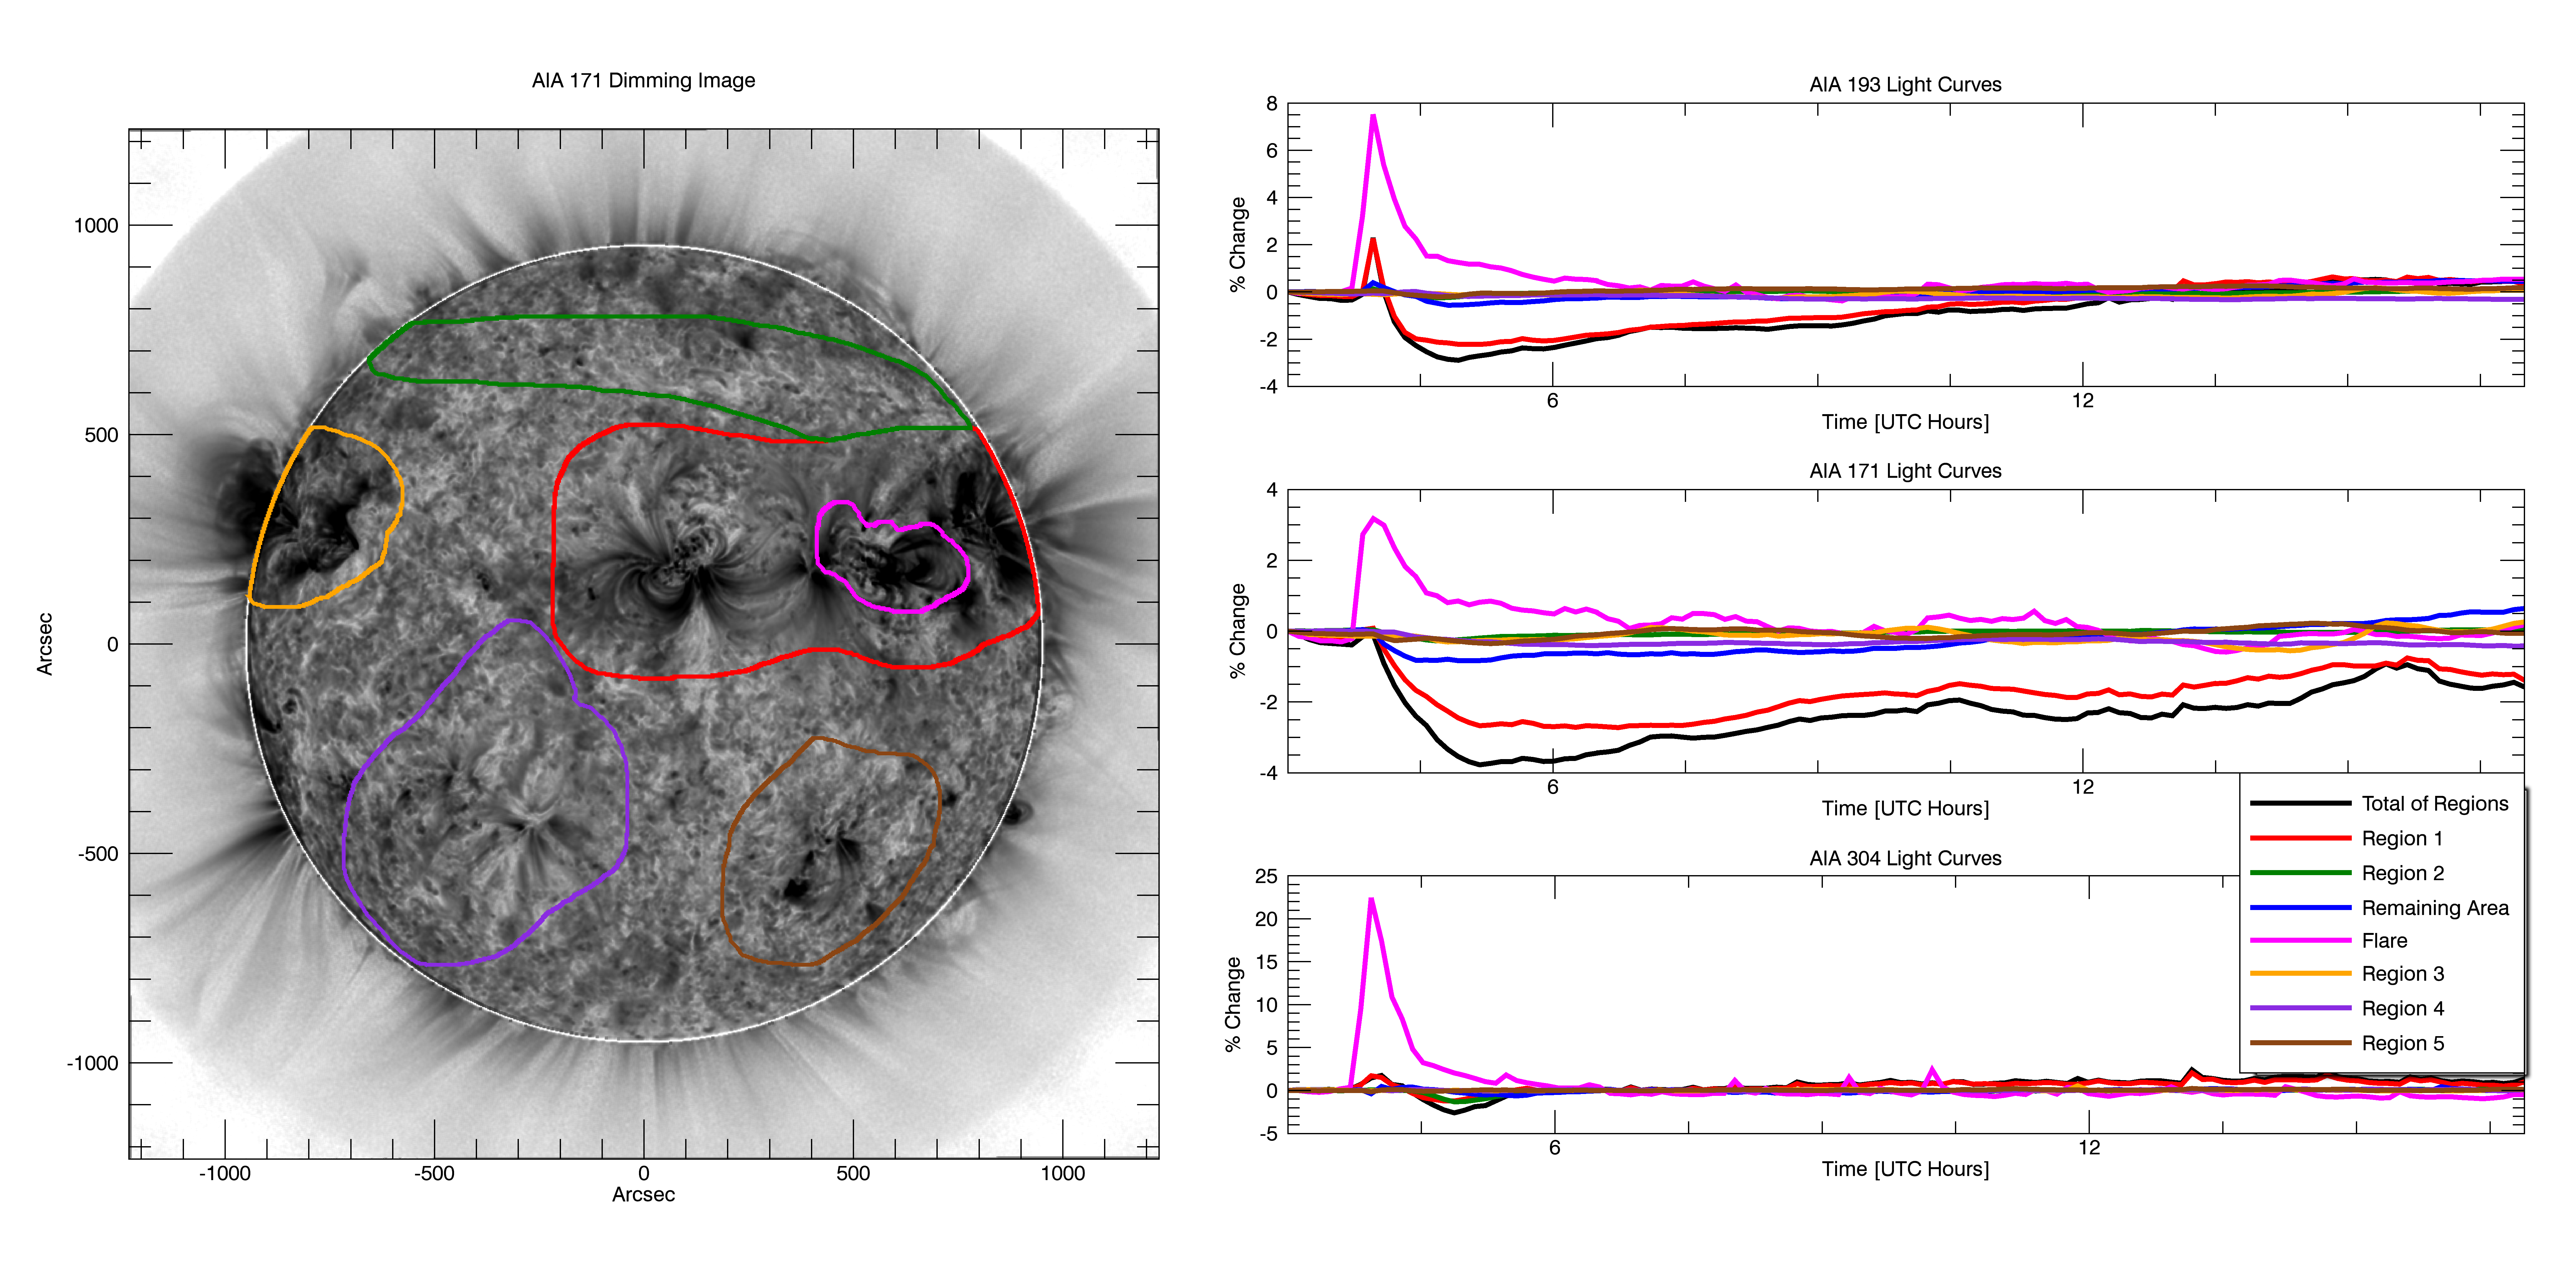
\includegraphics[width=166mm]{Images/Aia2011Aug4NewRegions.png}
    \end{center}
    \caption[Additional AIA contour analysis for 2011 August 4 event]{
        Same as Figure \ref{aia2011aug4} but with new contours selected and no point spread function correction applied. 
        Also 304 \AA\ data are now complete. 
	}
    \label{aia2011aug4newregions}
\end{figure}

Figure \ref{aia2011aug4newregions} is the same format as Figure \ref{aia2011aug4} but with different regions selected, and does not use images corrected with the point spread function. The latter explains why the total dimming is about 2\% less than in Figure \ref{aia2011aug4}. Of importance here is that the red contour, which encompasses the core dimming region from Figure \ref{aia2011aug4} and the most nearby non-flaring active region, accounts for the majority of total dimming in 193 \AA\ and 171 \AA. These two active regions are so close together that it is possible that the CME pulled mass away from a coronal volume encompassing both active regions. It can also be seen that 171 \AA\ has a more prominent dimming in the remaining area (blue), i.e. quiet-Sun, than in 193 \AA. This is evidence of heat-wave dimming described in \citet{Robbrecht2010}. 

Also note that while the AIA 193 \AA\ band contains the Fe XXIV 192 \AA\ emission line, this high ionization state is only expected in hot plasma such as in flaring loops, which are spatially isolated in the contours of Figures \ref{aia2010aug7}, \ref{aia2011aug4}, and \ref{aia2011aug4newregions}. Thus, for this particular case of spectral blending, the impact on analysis and interpretation is minimized. 

\begin{figure}[!h]
    \begin{center}
	    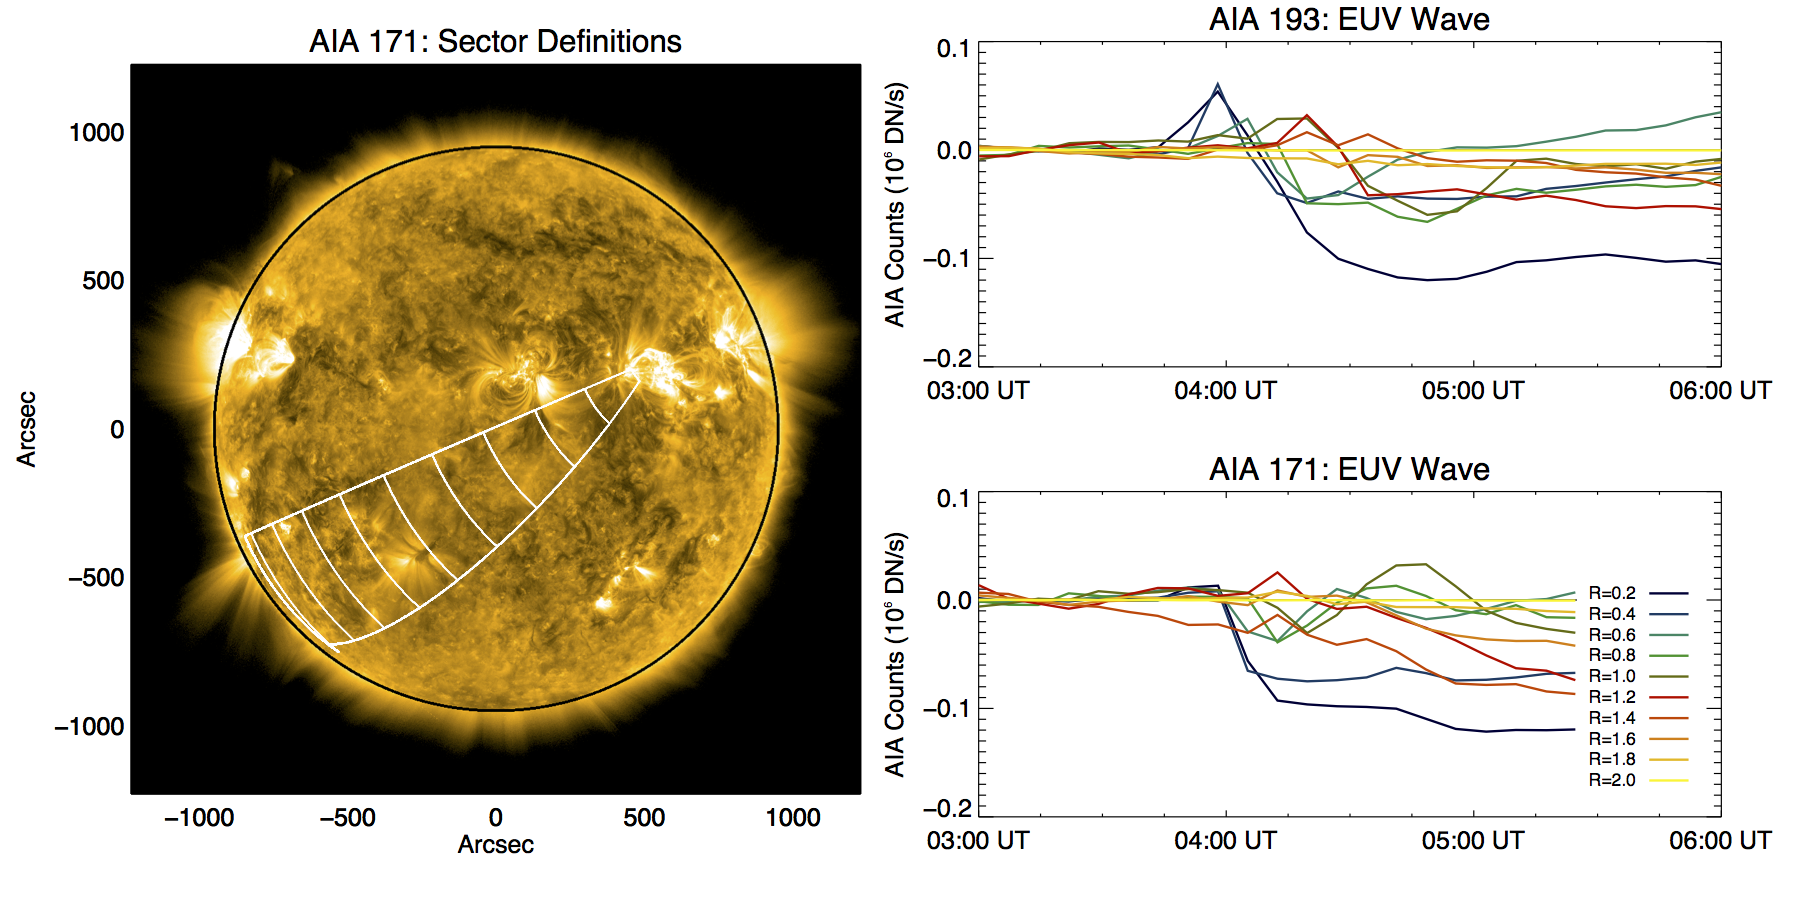
\includegraphics[width=166mm]{Images/Aia2011Aug4Wave.png}
    \end{center}
    \caption[AIA wave analysis for 2011 August 4 event]{
        Similar format to Figure \ref{aia2011aug4newregions}, but with geometric contours selected specifically for analysis 
        of propagating wave. In the line plots on the right, distance from the source active region increases with lightness
        of color. Figure courtesy of Rachel Hock. 
	}
    \label{aia2011aug4wave}
\end{figure}

Running-difference movies make viewing EUV waves easier but it is difficult get the same clarity with static images. Instead, Figure \ref{aia2011aug4wave} follows a similar format to earlier AIA figures but draws geometric contours propagating from the source active region. The light curves in Figure \ref{aia2011aug4wave} are color coded from dark to light corresponding to increasing distance from the source region. The propagation of the wave can be seen as the dark curves reach their minimum earlier with larger magnitude and the lightest curves show only a minor impact from the wave. This is expected behavior for any impulsive wave phenomenon as energy is dissipated in the surrounding medium. 

\paragraph{SDO/EVE EUV Irradiance Observations}
Figure \ref{eve2011aug4} shows selected extracted emission lines from EVE for the 2011 August 7 complex eruptive event. Because obscuration dimming is important for this case, the plot includes two He II lines: 256 \AA\ and 304 \AA, both of which show dimming at approximately the same time as what was seen in AIA (Figure \ref{aia2011aug4}). The irradiance increase from roughly 5:00 to 7:00 UT in Fe XIV 211 \AA\ may relate to the EUV late phase discussed in \citet{Woods2011}. Dimming in Fe IX to Fe XIII was significant in this case, roughly twice as large as in the simpler 2010 August 7 event. Furthermore, the peak time versus ionization state trend is reversed compared to the simpler event e.g., Fe IX 171 \AA\ actually peaks just prior to the GOES event peak time (second vertical dash), and higher ionization states peak later and later. This is indicative that heating processes are dominating the overall irradiance. In either heating or cooling cases, the flare-dimming deconvolution method discussed in Section \ref{sec:deconvolve} works equally well. 

\newpage
\begin{singlespace}
\begin{figure}[H]
    \begin{center}
	    \includegraphics[width=166mm]{Images/Eve2011Aug4.png}
    \end{center}
    \caption[EVE selected extracted emission lines for 2011 August 4 event]{
        Same as Figure \ref{eve2010aug7} but for the 2011 August 4 event, and showing He II 256 \AA\ and 304 \AA\ instead 
        of Fe XVI 335 \AA\ and Fe XVIII 94 \AA. Just as before, Fe IX to Fe XIII show clear 
        dimming, Fe XIV is borderline, and Fe XV to Fe XX show smooth brightening with no dimming. The Fe XX 131 \AA\ 
        profile is 3x larger than GOES 1-8 \AA\ but still has a similar shape and timing. Also note the 
        vertical axes: dimming is 2x larger than it was for the 2010 August 7 event. The two He II lines show dimming as 
        well, suggestive of obscuration dimming. 
	}
    \label{eve2011aug4}
\end{figure}
\end{singlespace}

\section{Flare-Dimming Deconvolution Method}
\label{sec:deconvolve}
Figures \ref{eve2010aug7} and \ref{eve2011aug4} showed how cooling and heating impact the time of an irradiance peak in each ionization state of Fe: cooling causes the low ionization states to peak later and heating causes the reverse. In either case, it is clear that dimming magnitude decreases with higher ionization states of Fe. Eventually, around Fe XIV at 211 \AA, dimming is no longer clear. The next ionization state, Fe XV at 284 \AA, shows strong brightening in response to the flare but no dimming. The shape of the flare peak is similar in all wavelengths\footnote{Though the shape of the flare peak appears to become more smooth at higher ionization states because of the significantly larger increase making the small oscillations imperceptible in the plots}. Using this observation, we developed a simple algorithm to remove the flare peak in the dimming lines. We make the assumption that the peak in the high ionization states is a good proxy for what \textit{would have} been observed in the low ionization states if there were no dimming. However, the magnitudes and timing are quite different. To account for this, we scale the larger peak down and shift it in time so that they are matched. An example of the process is shown in Figure \ref{flaredimmingdeconvolution} and a flow-chart of the algorithm is shown in Figure \ref{flaredimmingdeconvolutionalgorithm}. The ten-second EVE data are averaged to two-minutes to reduce noise (see black line in Figure \ref{flaredimmingdeconvolution}) and the simple IDL \textit{max} function applied to find the peak in the light curve for every emission line listed in Table \ref{tab:emissionlines}. Then, the scaled non-dimming emission line is shifted in time such that its peak matches the one in the dimming line (see green line in Figure \ref{flaredimmingdeconvolution}). Finally, the scaled and time-shifted non-dimming light curve is subtracted from the dimming emission line (see blue line in Figure \ref{flaredimmingdeconvolution}). 

\begin{figure}[!h]
    \begin{center}
	    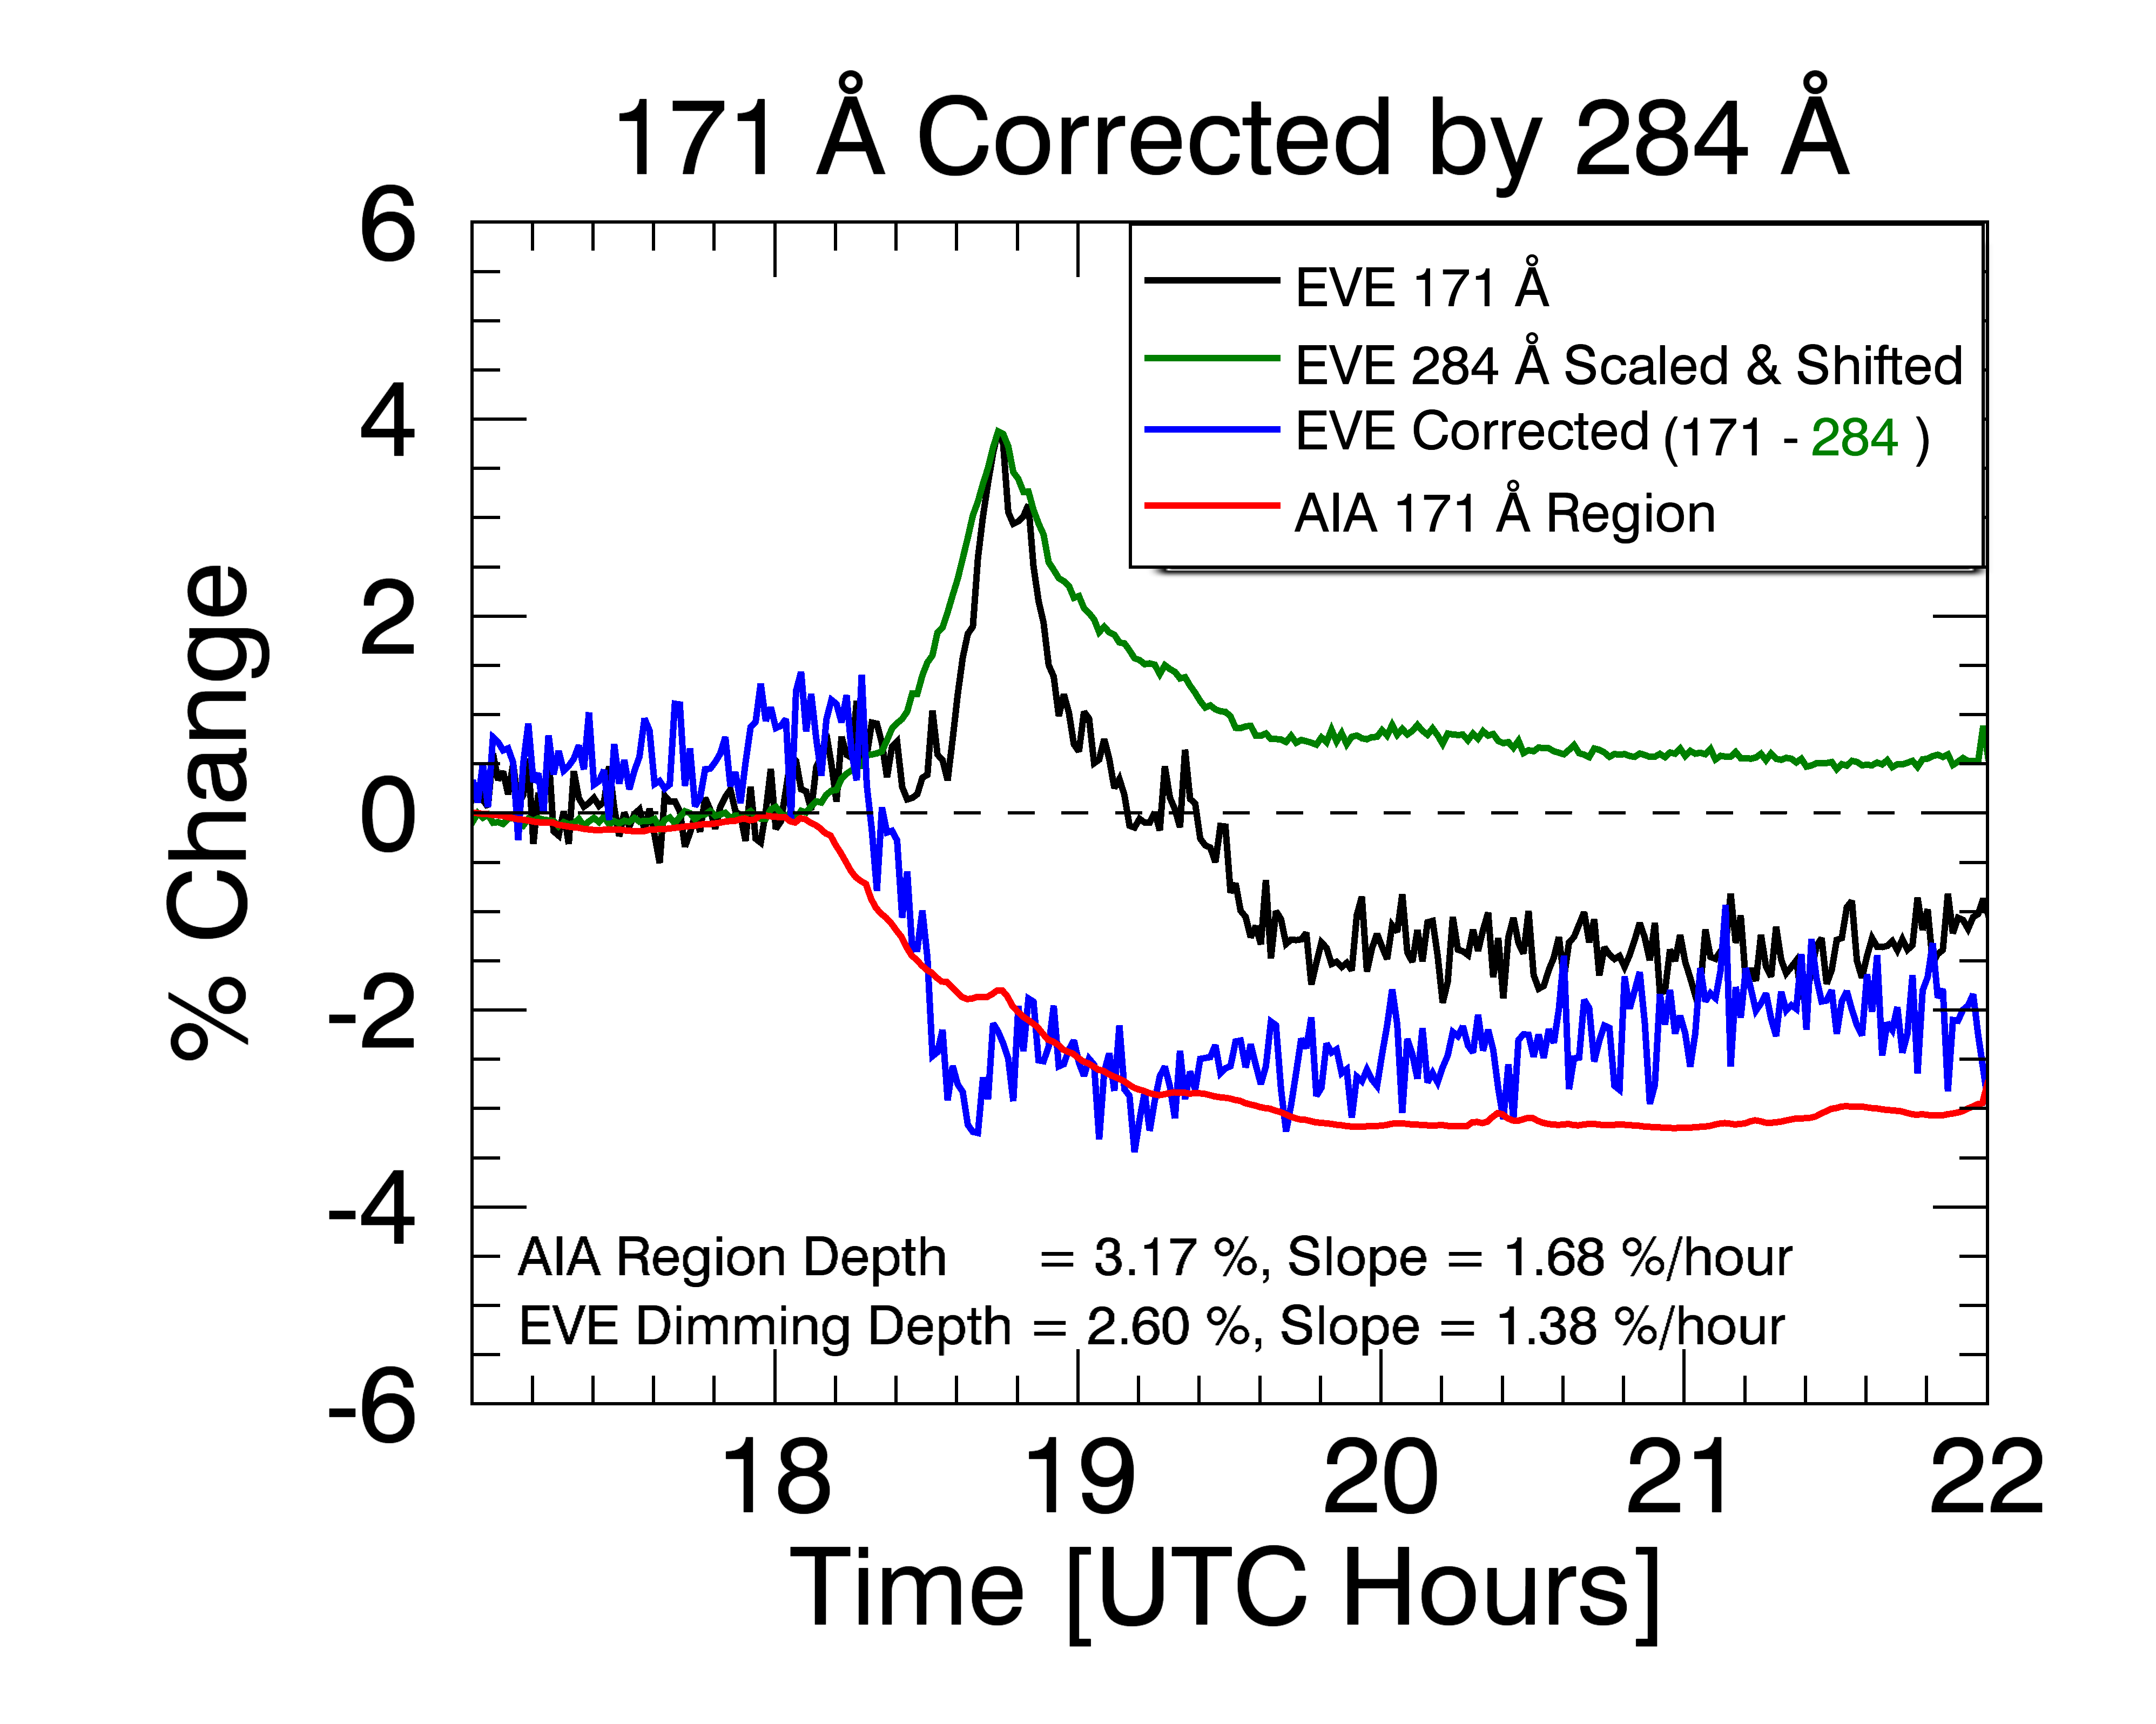
\includegraphics[width=100mm]{Images/DimmingCorrectionProcedure.png}
    \end{center}
    \caption[Flare-dimming deconvolution method example]{
        Example of the flare-dimming deconvolution method. This particular event is the simple case described in 
        Section \ref{sec:observationssimple}. A non-dimming line (e.g., 284 \AA) is scaled down and shifted in 
        time such that its flare peak matches the one in a dimming line (green and black, respectively). The scaled and 
        time-shifted non-dimming light curve is then subtracted from the dimming light curve, resulting in a "corrected" or
        "deconvolved" light curve representative of mass-loss dimming (blue). The red line is the same as the red line in 
        Figure \ref{aia2010aug7}, indicating the spatially isolated dimming in AIA 171. Dimming depth and slope are shown
        at the bottom of the plot and were computed at a particular time and time range, respectively. 
	}
    \label{flaredimmingdeconvolution}
\end{figure}

\begin{figure}[!h]
    \begin{center}
	    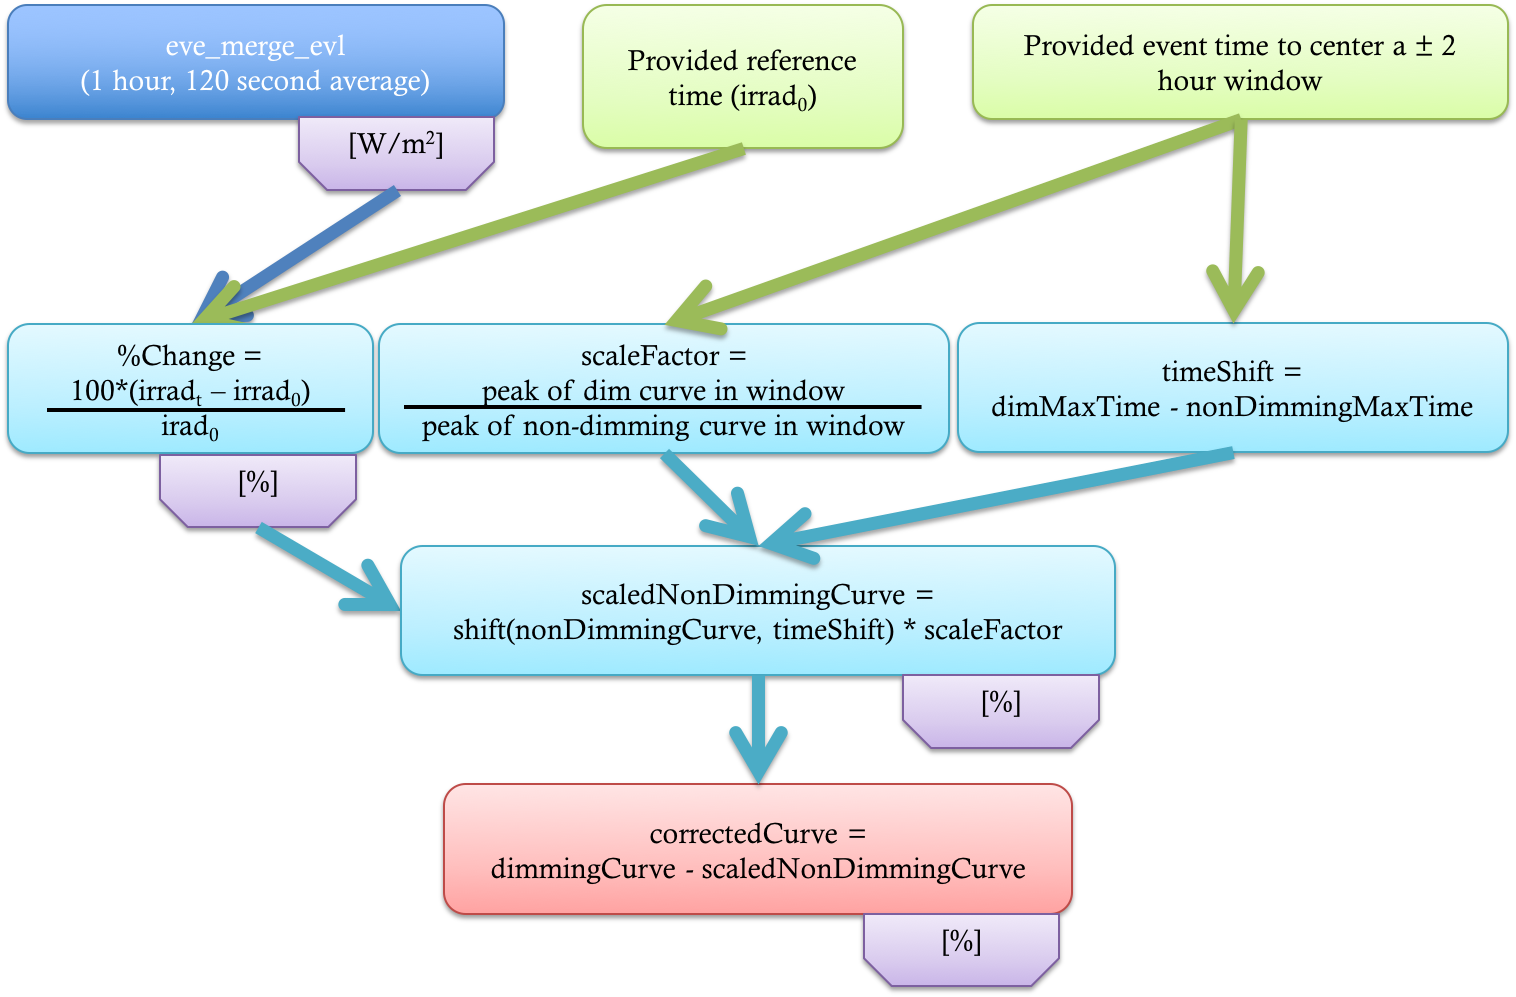
\includegraphics[width=160mm]{Images/DeconvolutionMethod.png}
    \end{center}
    \caption[Flare-dimming deconvolution algorithm schematic]{
        Flow-chart for the flare-dimming deconvolution algorithm. Rounded-rectangular boxes describe the steps and the 
        purple boxes indicate the units of the irradiance at that step. 
   	}
    \label{flaredimmingdeconvolutionalgorithm}
\end{figure}


The red line in Figure \ref{flaredimmingdeconvolution} is the same red line that was in Figure \ref{aia2010aug7}, which corresponded to the dimming area in AIA thought to be most associated with mass-loss from the corresponding observed CME. It is clear that the deconvolution method applied brings the EVE light curve much closer (from black line to blue line) to the AIA one (red line). The agreement is not perfect, particularly at later times, and the noise in EVE is greater -- even with the two-minute averaging -- than AIA. However, the agreement during the initial decline is much better and is where the slope of dimming is computed, which will be shown to be a critical proxy to CME velocity. The later rise in the corrected EVE line (blue) is due to a slow decrease in the scaled \& time-shifted correction line (green). The unaltered dimming line (black) is relatively flat in the later hours of the dimming, consistent with the AIA light curve (red). This behavior varies by event but a ``bottomed-out" dimming is common. Typically, the maximum depth is reached quickly and maintained for several hours. It will later be shown that depth is another critical proxy for CMEs; this one for CME mass. In practice, the depth is measured at a point soon after the maximum dimming is reached, so later behavior of the corrected EVE line (blue) is of less importance than the removal of the flare peak. The further in time one goes, the more likely it is for other events or physical processes to occur that would complicate the spatially-integrated EVE analysis. Duration of dimming may be an interesting parameter to study, but due to the continuing evolution and dynamics of the sun it is of secondary priority. Additionally, the duration is likely to be most closely linked to the physical processes responsible for filling plasma back into the void, relaxation of the disturbed system, and temperature evolution causing changes to ionization fractions. All of these have a tenuous connection to CME kinetics and thus provide less promise of providing a physical justification for dimming proxies for CMEs. 

Which combinations of dimming and non-dimming line make for the best dimming-isolated light curve? In the simple 2010 August 7 event, it was Fe IX 171 \AA\ (dimming) and Fe XV 284 \AA, respectively. In the 28 other cases studied (see Chapter \ref{chapterstatistical}), this same combination proved best. 

\section{Error Propagation}
\label{sec:deconvolveerrors}
Coronal dimming is a transient event lasting several hours that is studied in terms of relative change from the initiation time. As such, no long-term degradation of EVE needs to be factored into uncertainties i.e. the absolute accuracy is not important but the measurement precision is. To estimate precision, a period of solar inactivity was analyzed: 2013 January 28 from 00:00 - 01:00 UT. The estimated precision of these 120-second averaged EVE line data was calculated as the variance of the mean \citep{Bevington2003}, i.e., the standard deviation divided by the square root of the number of samples, which was 12 in this analysis. Table \ref{tab:evelineprecision} provides the estimated precision for each emission line used in this study, and provides a sense of how well we can detect EVE dimmings that typically have depths less than 5\% of the pre-flight irradiance level.

\begin{table}[!h]
    \caption[EVE precision by emission line]{
    Estimated precision for selected emission lines in EVE spectra. The Fe IX 171 \AA\ and Fe XV 284 \AA\ emission lines
    are the choice lines for dimming analysis.  
    }
    \begin{center}
    \begin{tabular}{|l|l|l|} \hline
	Ion & Wavelength (\AA) & Estimated Precision (\%) \\ \hline \hline
	Fe IX & 171 & 0.06 \\ \hline
	Fe X & 177 & 0.05  \\ \hline
	Fe XI & 180 & 0.04 \\ \hline
	Fe XII & 195 & 0.04 \\ \hline
	Fe XIII & 202 & 0.04 \\ \hline
	Fe XIV & 211 & 0.07 \\ \hline
	Fe XV & 284 & 0.08 \\ \hline
	Fe XVI & 335 & 0.17 \\ \hline
	Fe XVIII & 94 & 0.08 \\ \hline
	Fe XX & 132 & 0.20 \\ \hline
	\end{tabular}
    \\ \rule{0mm}{5mm}
    \end{center}
    \label{tab:evelineprecision}
\end{table}

These base uncertainties were propagated through each step of the EVE dimming correction method described in Section \ref{sec:deconvolve}. First, the line precisions are combined with the provided reference time to compute percent change (see Figure \ref{flaredimmingdeconvolutionalgorithm}, Equation \ref{eq:percentchange}). 

\begin{equation} 
    \% change = 100 \times \frac{(irrad_t - irrad_0)}{irrad_0}
    \label{eq:percentchange}
\end{equation}

\noindent where $irrad_t$ is the irradiance at each time and $irrad_0$ is the irradiance at the provided reference time. In practice, the latter is a manually selected pre-flare point that appears to correspond well to a quiet or well-behaved period. All of the uncertainty derivations to follow are based on the basic uncertainty propagation equation, 

\begin{gather}
    F = f(X,Y) \\
    \sigma^2_F = \sigma^2_x(\frac{\partial F}{\partial X})^2 + \sigma^2_Y(\frac{\partial F}{\partial Y})^2
    \label{eq:genericuncertainty}
\end{gather}

\noindent where $F$ is a generic function that will be specified for each of the steps of the deconvolution method. The first step of computing percent change (i.e. where F = Equation \ref{eq:percentchange}) has the corresponding uncertainty derivation: 

\begin{gather*} 
    \frac{\partial F}{\partial X} = \frac{100}{irrad_0} \implies 
    (\frac{\partial F}{\partial X})^2 = (\frac{100}{irrad_0})^2 \\    
    \frac{\partial F}{\partial Y} = -\frac{100 \times irrad_t}{irrad_0^2} 
    \implies (\frac{\partial F}{\partial Y})^2 = (-\frac{100 \times irrad_t}{irrad_0^2})^2 \\
    \therefore \sigma^2_F = \sigma^2_x(\frac{100}{irrad_0})^2 + \sigma^2_y(-\frac{100 \times irrad_t}{irrad_0^2})^2
    \label{eq:percentchangeuncertaintyderivation}
\end{gather*}

\begin{equation}
    \implies \sigma _F = \sqrt{\sigma^2_x(\frac{100}{irrad_0})^2 + \sigma^2_y(-\frac{100 \times irrad_t}{irrad_0^2})^2}
    \label{eq:percentchangeuncertainty}
\end{equation}


\noindent where $\sigma _x$ is the precision of $irrad_t$ and $\sigma _y$ is the precision of $irrad_0$, which will be identical in this case since Equation \ref{eq:percentchange} refers to a single emission line. This is the uncertainty corresponding to $dimmingCurve$ and $NonDimmingCurve$. The next step in the algorithm (see Figure \ref{flaredimmingdeconvolutionalgorithm}) is to scale the $NonDimmingCurve$ irradiance so that the peaks of the dimming and non-dimming line have the same magnitude (both of which are now in \% units). The derivation for the corresponding uncertainty is, 

\begin{gather*}
    F = xy \\
    \frac{\partial F}{\partial x} = y , \frac{\partial F}{\partial y} = x
    \label{eq:scaledbrightcurvederivation}
\end{gather*}

\begin{equation}
    \therefore \sigma^2_F = \sigma^2_x y^2 + \sigma^2_y x^2 = \sigma^2_{scaledNonDimmingCurve}
    \label{eq:scaledbrightcurvestep1}
\end{equation}

\noindent where $x$ is the non-dimming light curve, $\sigma _x$ is the result of Equation \ref{eq:percentchangeuncertainty} (i.e. the $\sigma _F$ in Equation \ref{eq:percentchangeuncertainty}), $y$ is the scale factor (which is a single value), and $\sigma _y$ is derived as follows: 

\begin{gather*}
    \text{Let} \frac{d}{b} = \frac{dimCurve_{peak}}{nondimCurve_{peak}} = y \\
    \sigma^2_y = \sigma^2_d(\frac{1}{b})^2 + \sigma^2_b(-\frac{d}{b^2})^2 \\
    \therefore \sigma^2_y = (\frac{\sigma _d}{b})^2 + (\frac{\sigma _bd}{b^2})^2
    \label{eq:scalefactoruncertainty}
\end{gather*}

Thus we have the $scaledNonDimmingCurve$ and its associated propagated uncertainty. The final step is to apply the correction to the $dimmingCurve$, which is just a simple subtraction, resulting in the final uncertainty: 

\begin{equation}
    \sigma _{correctedCurve} = \sqrt{\sigma^2_{dimmingCurve} + \sigma^2_{scaledNonDimmingCurve}}
    \label{eq:correctedcurveuncertainty}
\end{equation}

\noindent where $\sigma^2_{dimmingCurve}$ comes from Equation \ref{eq:percentchangeuncertainty} and $\sigma^2_{scaledNonDimmingCurve}$ comes from Equation \ref{eq:scaledbrightcurvestep1}. Evaluation of Equation \ref{eq:correctedcurveuncertainty} with EVE data results in an uncertainty of ~$\pm$ 0.175\%\footnote{\%\ here is the same unit as the irradiance, not a percentage of the irradiance value}. Chapter \ref{chapterstatistical} will discuss the passing of the above uncertainty into IDL's \textit{poly{\_}fit} function and the final resultant errors associated with that process. 

\section{Dimming Parameterization Results}
\label{sec:casestudyresults}

\subsection{Simple Dimming Case}
Parameterization of dimming is focused primarily on slope and depth, both of which are selected by eye. The time to select for these parameters is debatable but in this case, we chose depth to be a point soon after the dimming ``floor" is reached in AIA Region 1 (red contour and line). Slope was taken to this point, starting from 17:50 UT -- the time just before GOES 1-8 \AA\ and EVE 131 \AA\ began to rise. The deconvolution method (Section \ref{sec:deconvolve}) significantly reduces the impact of the flare’s gradual phase peak to dimming measurements for EVE. Prior to the correction, EVE would have measured a dimming depth of 1.27\% in 171 \AA\ and 0.18\% in 195 \AA. After the correction, these values are 2.94\% and 2.09\%, respectively. Similarly, slope was changed from 1 $\%\ hr^{-1}$ (171 \AA) and 0$\%\ hr^{-1}$ (195 Å) to 2.29$\%\ hr^{-1}$ (171 \AA\ corrected) and 2.09$\%\ hr^{-1}$ (195 \AA\ corrected). Furthermore, if this event was being observed in real time, the gradual phase peak makes it impossible to estimate the amount and speed (slope) of dimming accurately. This correction method allows the irradiance increase due to the gradual phase contribution to be compensated in the EVE time series that have dimming.

\begin{figure}[!h]
    \begin{center}
	    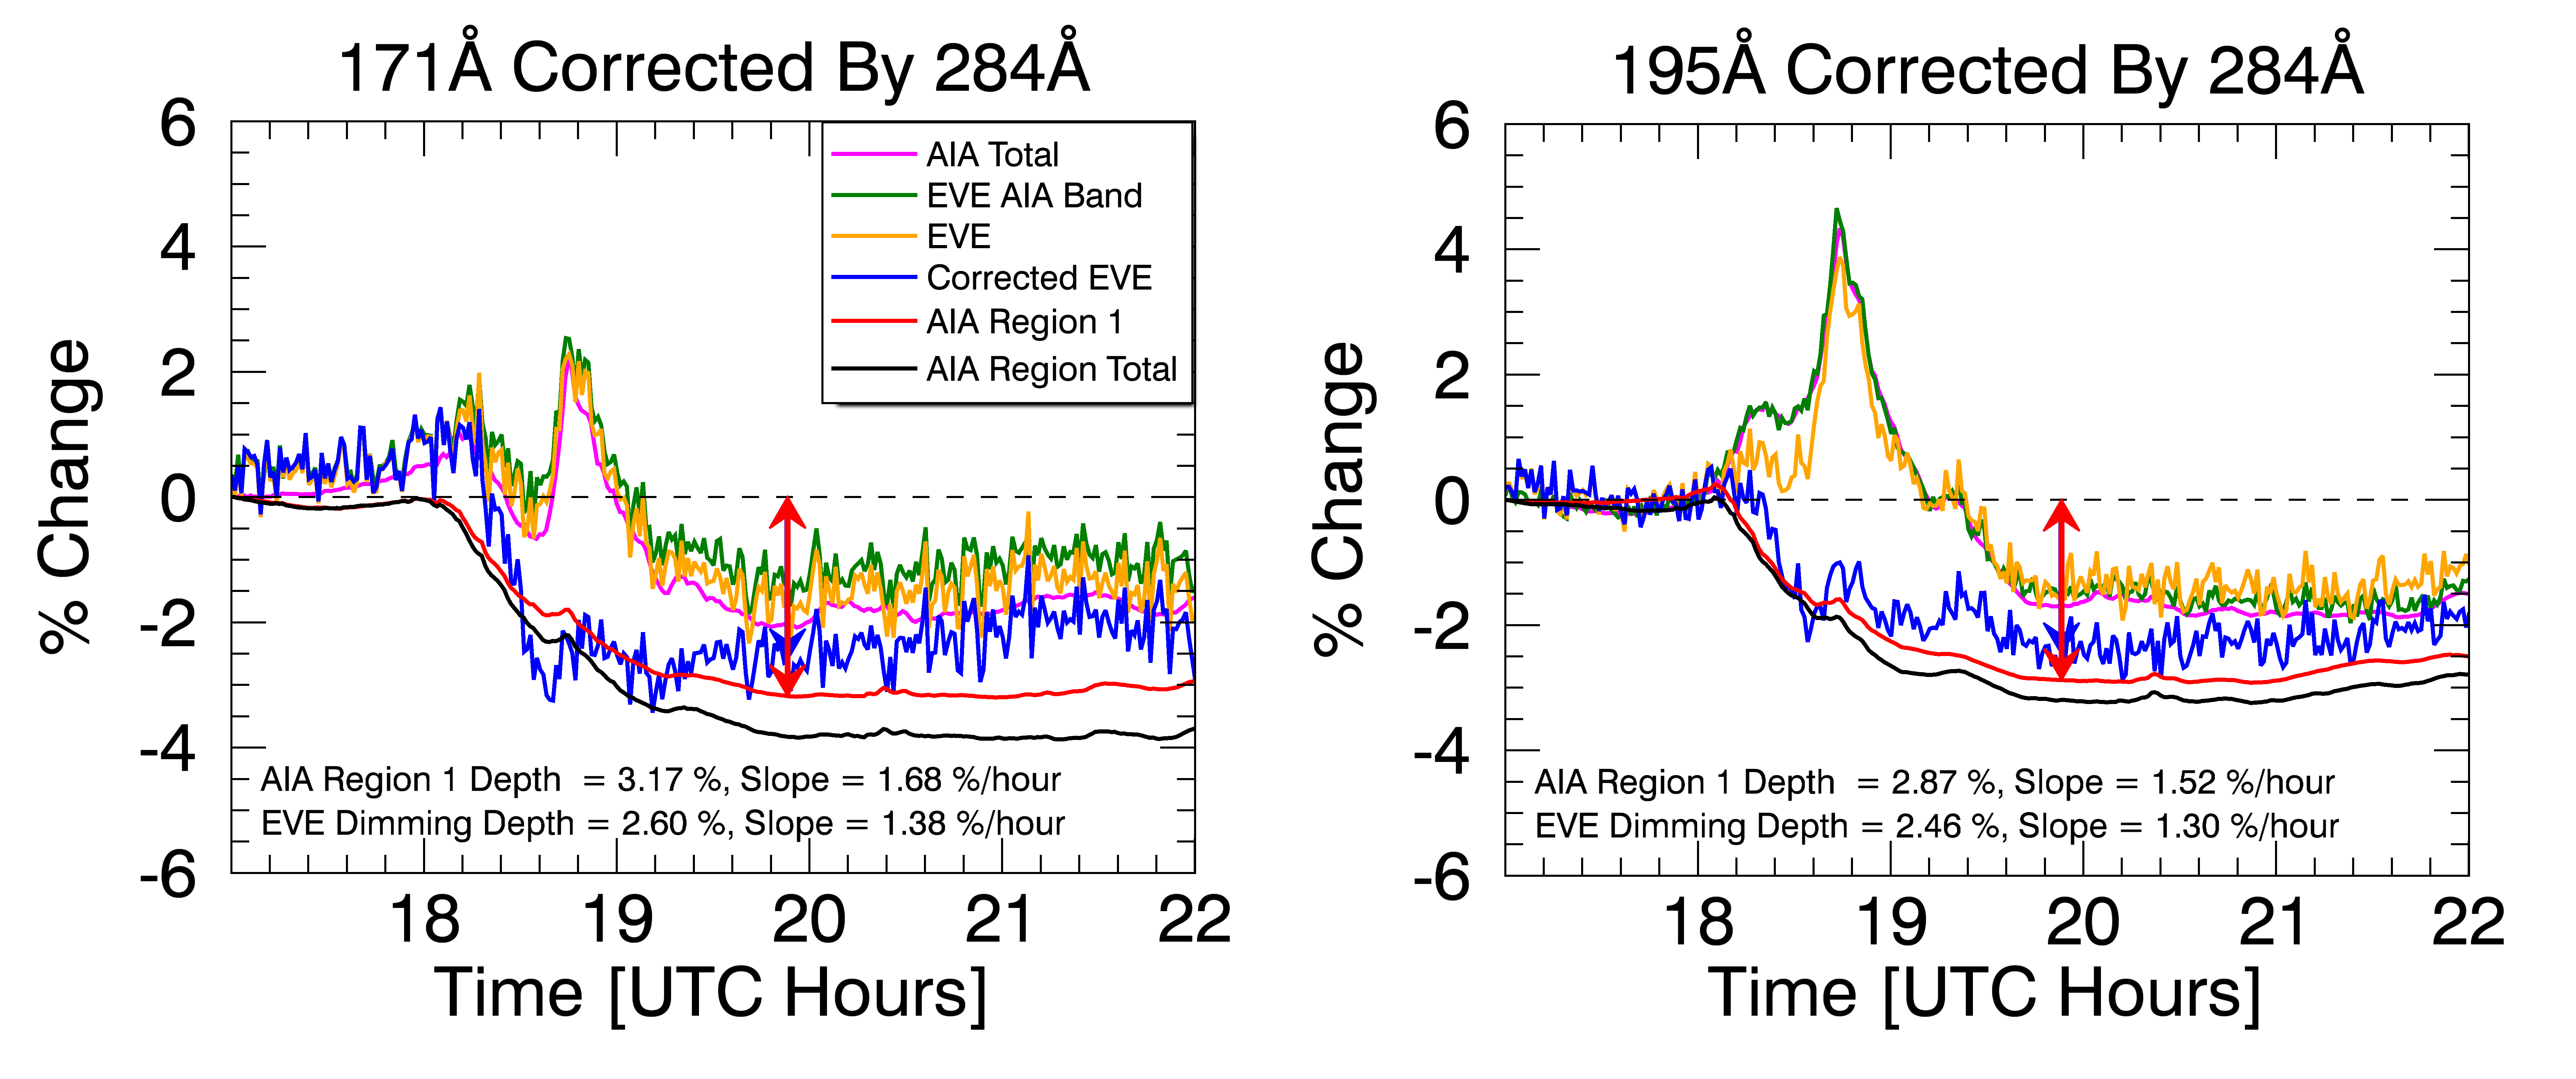
\includegraphics[width=166mm]{Images/EVECorrectionResults2010Aug7.png}
    \end{center}
    \caption[Dimming parameterization for 2010 August 7 event]{
        Both plots are similar to Figure \ref{flaredimmingdeconvolution} but provide more detail. The left shows results 
        from 171 \AA\ and the right is for 193 \AA\ (AIA) / 195 \AA\ (EVE). The red vertical arrow indicates the point 
        where depth is computed and overlaps a blue vertical arrow indicating the end time of slope computation. 
        The slope range begins at 17:50 UT. 
   	}
    \label{fig:parameterization2010aug7}
\end{figure}

The small difference in time between different emission peaks -- Fe XX peaks 21 minutes before Fe IX in this case -- is information that can be used to understand the temperature evolution during dimming. In this event, that time difference is significantly shorter than the hours-long duration of the total dimming event. Thus, it is unlikely that thermal dimming is a significant contributor to the total observed dimming. Instead, our correction method uses nondimming lines as independent measurements of the flare gradual phase profile. Since no dimming is observed in the nondimming lines, the gradual phase profile is assumed to be pure and can then be used as a proxy to remove only the effect of the gradual phase in the dimming light curve with a minimal impact on total dimming. In this way, we can effectively match AIA dimming observations, which are capable of isolating the flaring coronal loops.

The expectation is that the EVE-corrected dimming results should have the same amount of dimming as the AIA results and are also independent of Fe ionization level (in the dimming lines). Figure \ref{fig:parameterization2010aug7} shows the comparison of EVE-corrected dimming time series to AIA results in both 171 \AA\ and 193/195 \AA, and Table \ref{tab:dimmingresults2010aug7} lists the dimming results. 

\begin{table}[!h]
    \caption[Key dimming results for 2010 August 7 event]{
        Key dimming results for 2010 August 7 event. Note that 195 \AA\ in EVE corresponds to the 193 \AA\ band in AIA, 
        which encompasses 195 \AA. 
    }
    \begin{center}
    \begin{tabular}{|p{1cm}|p{1cm}|p{1.2cm}|p{1.8cm}|p{1.8cm}|p{1.4cm}|p{1.4cm}|p{1.7cm}|p{1.7cm}|} \hline
	Dim line (\AA) & AIA Total Depth (\%) & AIA Reg. 1 Depth (\%) & EVE Depth Corrected (\%) & EVE Depth Uncorrected (\%) & AIA Total Slope ($\%\ hr^{-1}$) & AIA Rg. 1 slope ($\%\ hr^{-1}$) & EVE Slope Corrected ($\%\ hr^{-1}$) & EVE Slope Uncorrected ($\%\ hr^{-1}$) \\ \hline \hline
	171 & 2.03 & 3.17 & 2.60 & 1.63 & 1.07 & 1.68 & 1.38 & 0.86 \\ \hline
	177 & -- & -- & 2.79 & 1.89 & -- & -- & 1.48 & 1.00 \\ \hline
	180 & -- & -- & 2.87 & 1.98 & -- & -- & 1.52 & 1.05 \\ \hline
	195 & 1.68 & 2.87 & 2.46 & 1.52 & 0.89 & 1.52 & 1.30 & 0.81 \\ \hline
	202 & -- & -- & 2.31 & 1.60 & -- & -- & 1.22 & 0.85 \\ \hline
	211 & 0.52 & 2.03 & 2.57 & 1.60 & 0.28 & 1.50 & 1.36 & 0.85 \\ \hline
	\end{tabular}
    \\ \rule{0mm}{5mm}
    \end{center}
    \label{tab:dimmingresults2010aug7}
\end{table} 

AIA Region 1 is considered the reference for mass-loss dimming, so its dimming depth and slope are compared as an estimate of uncertainty for these results from EVE. The differences for the AIA 171 \AA\ and 195 \AA\ dimming depth and slope are 0.3\% and 0.16$\%\ hr^{-1}$, respectively. The relative uncertainty of these is 10\% of the mean depth and slope values, being 3.02\% and 1.60$\%\ hr^{-1}$. These differences in the two different AIA bands could reflect the uncertainty that Region 1 is only due to mass-loss dimming and our ability to identify the best Region 1 boundary to encompass the mass-loss dimming phenomena. However, selecting a slightly different boundary did not greatly impact the resultant light curves, so the difference may be real. This would indicate that AIA too sees shallower dimming for higher ionization states if the deconvolution method described in Section \ref{sec:deconvolve} is not applied. The corrected EVE results for dimming depth and slope have mean values of 2.53\% and 1.34$\%\ hr^{-1}$, and both are 14\% less than the AIA Region 1 mean values. The standard deviations for the six EVE lines’ corrected dimming depth and slope are 0.21\% and 0.11$\%\ hr^{-1}$, respectively. As expected (intended), the EVE corrected results are much more self-consistent with each other than the uncorrected results. The slope tracks the depth variation well; that is, the slope is less when the depth is less. Our expectation was that the slope could represent the CME velocity, and the depth could represent the CME mass loss. 

\subsection{Complex Dimming Case}

\begin{figure}[!h]
    \begin{center}
	    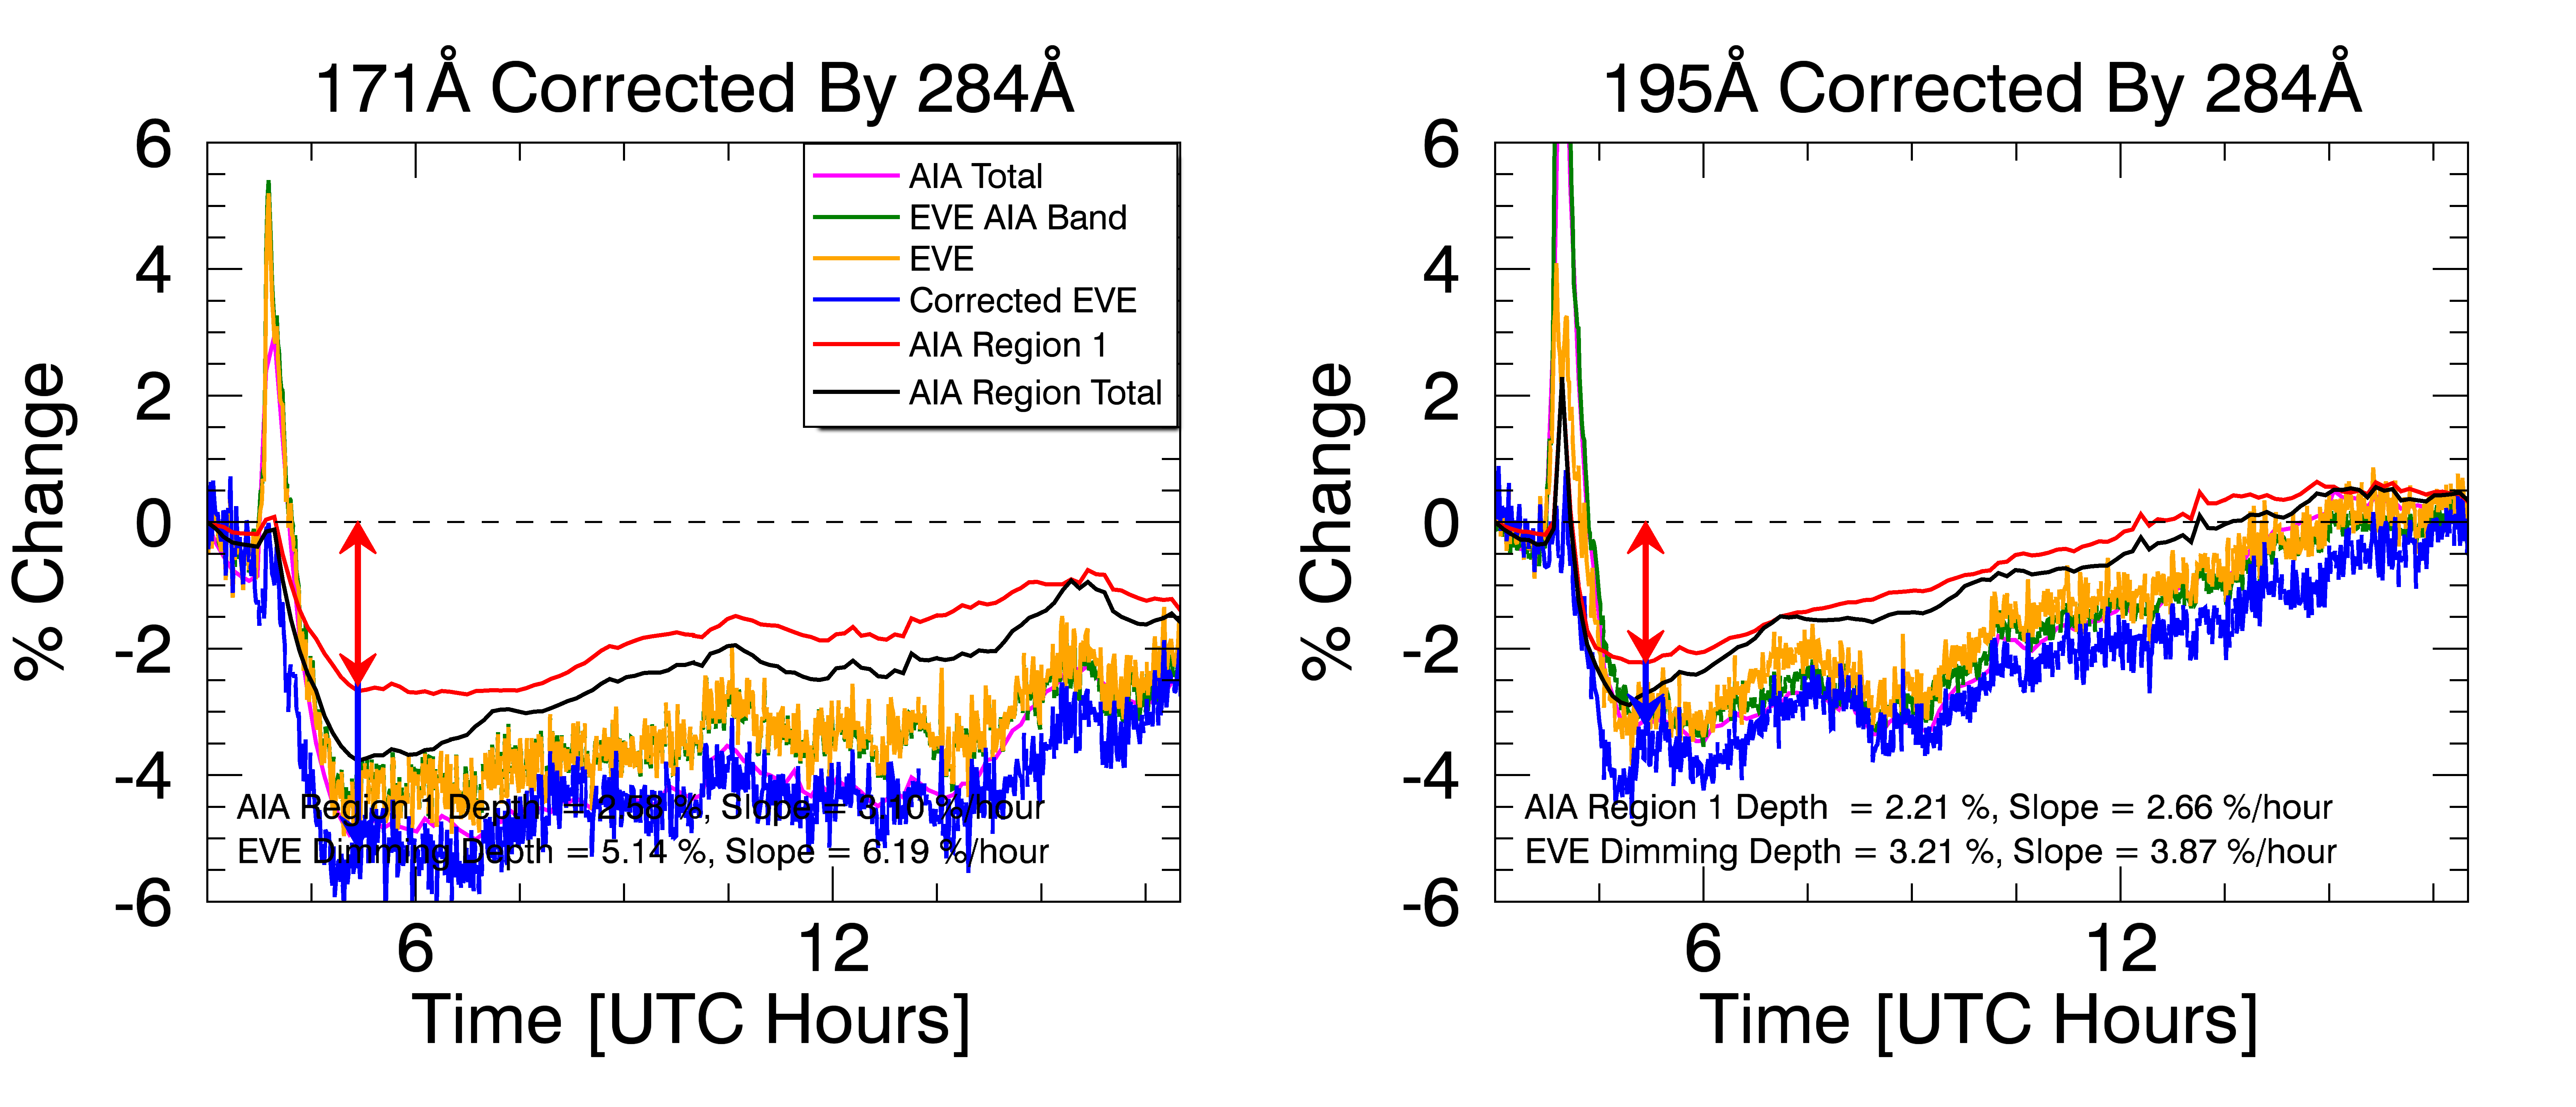
\includegraphics[width=166mm]{Images/EveCorrectionResults2011Aug4.png}
    \end{center}
    \caption[Dimming parameterization for 2011 August 4 event]{
        Same as Figure \ref{fig:parameterization2010aug7} but for the 2011 August 4, more complex, case. The AIA regions
        correspond to those selected in Figure \ref{aia2011aug4newregions}. 
   	}
    \label{fig:parameterization2011aug4}
\end{figure}

The dimming parameterization method in this case was the same as in the simple dimming case above. Figure \ref{fig:parameterization2011aug4} shows the analogous plots for this event. While the general trend of EVE follows AIA, it's clear from these plots that applying the same deconvolution methods does not result in as good a match of EVE to AIA. Note that even uncorrected EVE reaches a deeper minimum than the AIA light curves\footnote{Remember that the black line is the total inside contoured areas in AIA, not the total disk}. The only way for the deconvolution method to raise EVE irradiance would be for the nondimming line to have dimming, which would violate the definition. Since this was not the case, all of the corrected/deconvolved EVE light curves (blue) are even lower than the uncorrected EVE dimming line (gold), bringing it further from the AIA "core dimming" light curve (red). Nevertheless, the deconvolution method did successfully remove the flare peak in dimming lines as can be seen in the difference between the raw EVE (gold) and corrected EVE (blue) light curves. AIA showed that the remaining area (i.e. quiet Sun) had non-negligible dimming (black curve in Figure \ref{aia2011aug4} and blue in Figure \ref{aia2011aug4newregions}). Adding that to the AIA total dimming for 171 \AA\ would result in a peak dimming of about 4\% -- still 1\% lower than what is seen in EVE. Doing the same for 195 \AA\ would get the two to match within 1\%. The analysis is further complicated by the fact that the AIA bandpasses are several nanometers wide causing blending of many emission lines and continuum that makes direct comparison with EVE difficult, particularly for an event with so many simultaneous physical processes involved, each of which has an impact on the irradiance that can vary through time. 

The ultimate goal of the dimming analysis is to provide proxies for CME mass and velocity. This event was included in the semi-statistical study to determine the relationship between those CME parameters and the dimming depth and slope that will be discussed in Chapter \ref{chapterstatistical}. 


\section{Case Studies Summary}
To summarize the physical processes taking place in the simpler 2010 August 7 event, the plasma and its irradiance have source and sink terms. Near the beginning of the flare, heating is very dominant and causes a rapid increase in high ionization states for the various Fe emissions. Later in the flare, cooling of the plasma causes an increase in lower ionization states, and those cooler lines peak later than the hot lines. Through it all, the mass ejection can act as a sink for most coronal emissions. Early in the flare, before the low ionization states have been strongly affected by the cooling described above, the mass ejection dominates and causes the irradiance to visibly drop. Much later in the flare process, as the plasma approaches its preflare level, the missing plasma again becomes apparent in the irradiance time series as an hours-long, few-percent decrease. Quantitative dimming results are summarized in Table \ref{tab:dimmingresults2010aug7}. 

The physical interpretation of the more complex 2011 August 4 event is more difficult to obtain. The size of the flare was nearly an order of magnitude larger than in the simpler 2010 August 7 case and the associated CME velocity was 1.5x faster -- together, these are a general indicator that the amount of energy involved in the eruptive event was much larger in the more complex event. Additionally, the pre-eruption state of the Sun was more complex for the 2011 August 4 event, as evidenced by the more numerous active regions and polar filament, the coronal streamers, and the proximity of active regions to the one responsible for the eruption itself. All of this means that more energy was released via more mechanisms. The EUV wave was much more prominent in this case, sympathetic responses were clear, and heating (rather than cooling) dominated the irradiance indicative of energetic processes dominating relaxing ones. Quantitative dimming results are summarized in Table \ref{tab:aia2011aug4}. 